
%version 2: \usepackage{hyperref}


%%%%%%%%%%%%%%%%%%%%%%%%%%%%%%%%%%%%%%%%%%%%%%%%%%%%%%%%%%%%%%%%%%%%%%%%
%Para las ecuaciones siempre es Ec.(n).
%Para las figuras siempre es Fig.n, incluso en el caption de la figura. Tambien las Tablas
%Para las referencias es [n]
%%%%%%%%%%%%%%%%%%%%%%%%%%%%%%%%%%%%%%%%%%%%%%%%%%%%%%%%%%%%%%%%%%%%%%%%

\documentclass[
reprint,
%notitlepage,
%superscriptaddress,
%groupedaddress,
%unsortedaddress,
%runinaddress,
%frontmatterverbose, 
%preprint,
%showpacs,preprintnumbers,
%nofootinbib,
%nobibnotes,
%bibnotes,
%11 pt,
amsmath,
amssymb,
%aps,
%pra,
prb,
%rmp,
%tightenlines %esto hizo el milagro de sacar los espacios en blancos estocásticos (?)
%prstab,
%prstper,
%floatfix,\textbf{}
]{revtex4-1} %Instalar primero para usarlo. Paquete malo.

%\documentclass[onecolumn, aps, amsmath,amssymb ]{article}
\usepackage{lipsum}  
\usepackage{graphicx}% Include figure files
\usepackage{subfig}
\usepackage{braket}
\usepackage{comment} %comment large chunks of text
\usepackage{dcolumn}% Align table columns on decimal point
\usepackage{bm}% bold math
%\usepackage{hyperref}% add hypertext capabilities
\usepackage[mathlines]{lineno}% Enable numbering of text and display math
%\linenumbers\relax % Commence numbering lines
\usepackage{mathtools} %% Para el supraíndice

\usepackage[nice]{nicefrac}

%%%%%%%El Señor Español%%%%%%%%%%%%%%%%%%%%%%%%%%%
\usepackage[utf8]{inputenc} %acento
\usepackage[
spanish, %El lenguaje.
es-tabla, %La tabla y no cuadro.
activeacute, %El acento.
es-nodecimaldot %Punto y no coma con separador de números
]{babel}
\usepackage{microtype} %para hacerlo más bonito :33 como vos (?) 
%%%%%%%%%%%%%%%%%%%%%%%%%%%%%%%%%%%%%%%%%%%%%%%%%%%
%%%%%%%%% Para que las imágenes se queden dónde las quiero (?
\usepackage{float}
%%%%%%%%%%
\usepackage{enumitem}
\usepackage{hyperref} % Para usar \url

%%%%%%%%Cambia a Fig de Figure%%%%%%%%%%
\makeatletter
\renewcommand{\fnum@figure}{Fig. \thefigure} 
\makeatother
%%%%%%%%%%%%%%%%%%%%%%%%%%%%%%%%%%%%%%%%
\raggedbottom

\begin{document}

\title{Práctica 1: Redes Neuronales y Aprendizaje Profundo para Visión Artificial}
\author{Evelyn~G.~Coronel}

\affiliation{
Aprendizaje Profundo y Redes Neuronales Artificiales\\ Instituto Balseiro\\}

\date[]{\lowercase{\today}} %%lw para lw, [] sin date

\maketitle
%\onecolumngrid


\section*{Ejercicio 1}

En este ejercicio se implementó una regresión lineal de la  para un cantidad N de puntos en d dimensiones.  Para realizar este ejercicio se generan los valores de $x_i$ y $a_{m,exacto}$ de forma aleatoria entre $[-4,4]$. se calcula el valor
\begin{equation}
  y_i= \sum_{i=1}^d a_{i,esperado}x_i+ a_0 + \epsilon[-1,1]  
\end{equation}
donde se agrega un ruido uniforme que varía entre $[-1,1]$

Una vez obtenido el conjunto de datos $X$, se calculan  los parámetros esperados de la regresión lineal mediante la Ec.\,\ref{eq:ejer1}

\begin{equation}
     \vec a_{esperado} = (X^TX)^{-1}X^T \vec y,
     \label{eq:ejer1}
 \end{equation} 
donde $\vec a$ representa a $\{a_i, a_0 \}$, $X$ es la representación matricial de datos e $\vec y$ son los valores $y_i$.

En las Figs.  \ref{fig:ejer1_a_ejemplos} y \ref{fig:ejer1_y_ejemplos}  se muestran los errores cuadráticos medios  (MSE) en función de la cantidad de ejemplos dados para calcular los parámetros del problema así también de la salida.  Se observa como el error disminuye exponencialmente con la cantidad de datos.

Se observa  para una dimensión fija, el MSE disminuye a medida que se aumenta la cantidad de ejemplos para calcular los parámetros. En las mismas figuras se observa en subfigura donde se muestra como varía el valor de MSE fijando la cantidad de ejemplos, donde el error también aumenta con la dimensión, esto indica que a medida que voy a aumentando la dimensión del problema voy a necesitar más ejemplos para obtener un error menor. 
Como se muestra en las subfiguras, considerando la cantidad de ejemplos constante, los errores  aumenta con la dimensión. Más aún, si consideramos un valor de MSE fijo, por ejemplo en la Fig.\ref{fig:ejer1_y_ejemplos} con $MSE\approx 0.5$, con $d=80$ se necesitaron $\sim 180$ ejemplos para llegar a ese error,para  $d=120$ se necesitaron $\sim 270$ y para $d=160$ se necesitaron $\sim 380$  ejemplos. Por lo que se puede decir que:

\begin{equation}
    \Delta d \approx \Delta N  
\end{equation}
En el problema  de la dimensionalidad se espera que $\nicefrac{\Delta N}{\Delta  d}$ siga una forma exponencial. En este caso sigue un comportamiento lineal debido a que el problema que se trabaja es una regresión lineal. 



    \begin{figure}[H]
        \centering
        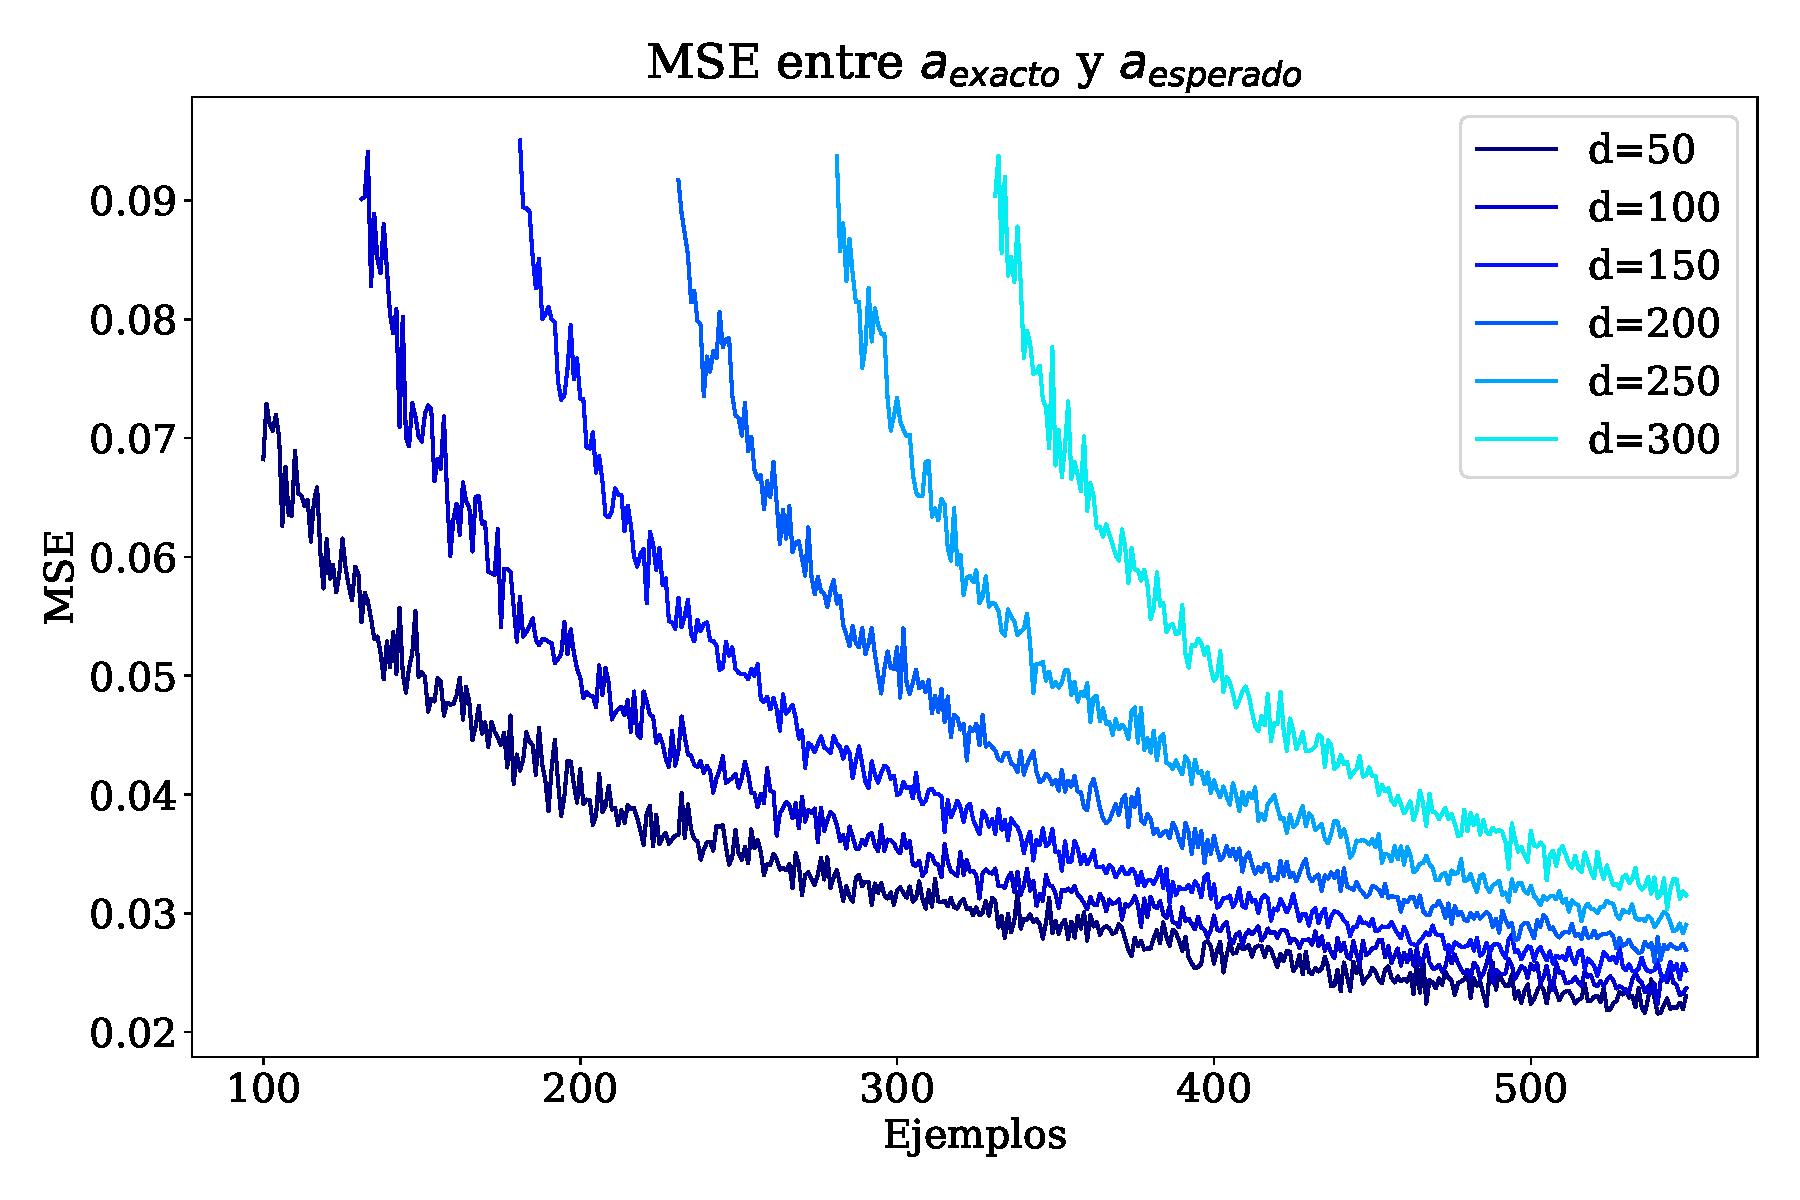
\includegraphics[width=0.5\textwidth]{plots/ejer_1_mse_a_ejemplos.pdf}
        \caption{MSE entre los parámetros exactos y obtenidos en función de los ejemplos de entrenamiento. También se muestra en la subfigura el comportamiento del MSE en función de la dimensión con cantidad de ejemplos fija.}
        \label{fig:ejer1_a_ejemplos}
    \end{figure}


    \begin{figure}[H]
        \centering
        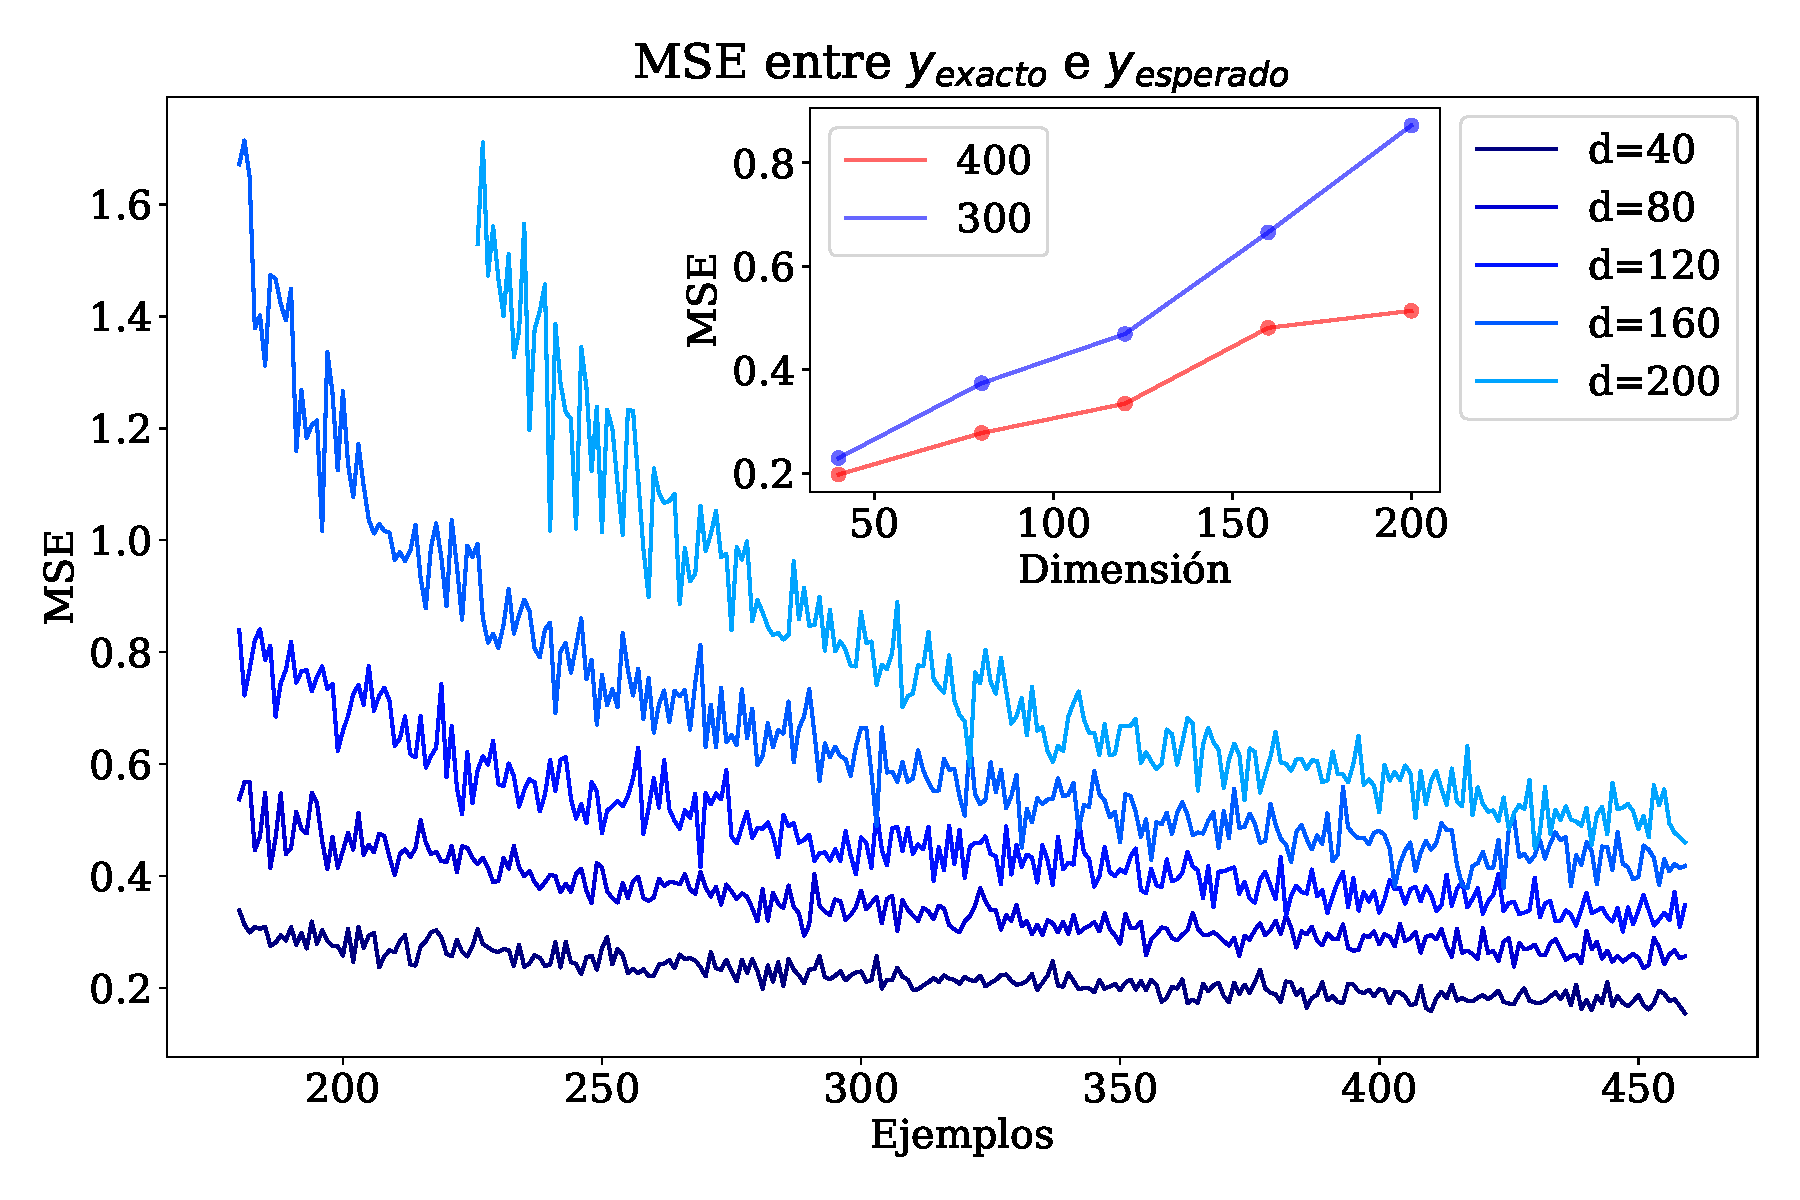
\includegraphics[width=0.5\textwidth]{plots/ejer_1_mse_y_ejemplos.pdf}
        \caption{MSE entre la salida $y_i$ exacta y la obtenida en función de los ejemplos de entrenamiento. Se  muestra la misma subfigura que la gráfica anterior.}
        \label{fig:ejer1_y_ejemplos}
    \end{figure}

    \section*{Ejercicio 2}

    En este ejercicio se generó un conjunto de datos en dimensión $d=7$ distribuidos en $p=4$ distribuciones normales con media y desviación estándar aleatorias entre $[-3, 3]$ y $[0.3,1.3]$ respectivamente.   Sobre este conjunto se implemente el algoritmo de \emph{k-means} para clasificar a los puntos en $4$ grupos.
    
    El algoritmo usa la media del grupo, o centroide, para definir si un punto pertenece o no al grupo. Para empezar el algoritmo se inicializan los centroides con puntos aleatorios del conjunto de datos.  A medidas que se realizan las iteraciones, los centroides tienden a las medias que se utilizaron para la inicialización de los datos, esto es propio a la forma con la que se generan los puntos para clasificar.

    Dependiendo del conjunto de datos y de los centroides iniciales, el algoritmo puede converger a una solución coherente o no. En  la Fig.\,\ref{fig:ejer2_converge} se muestra dos estados de la clasificación, la imagen superior es el estado iniciales de los puntos, con la clasificación y centroides aleatorios, mientras que en la imagen inferior se observa el estado final de las iteraciones donde los centroides calculados por el algoritmo convergen a la media de la distribuciones normales del conjunto.

    \begin{figure}[H]
        \centering
        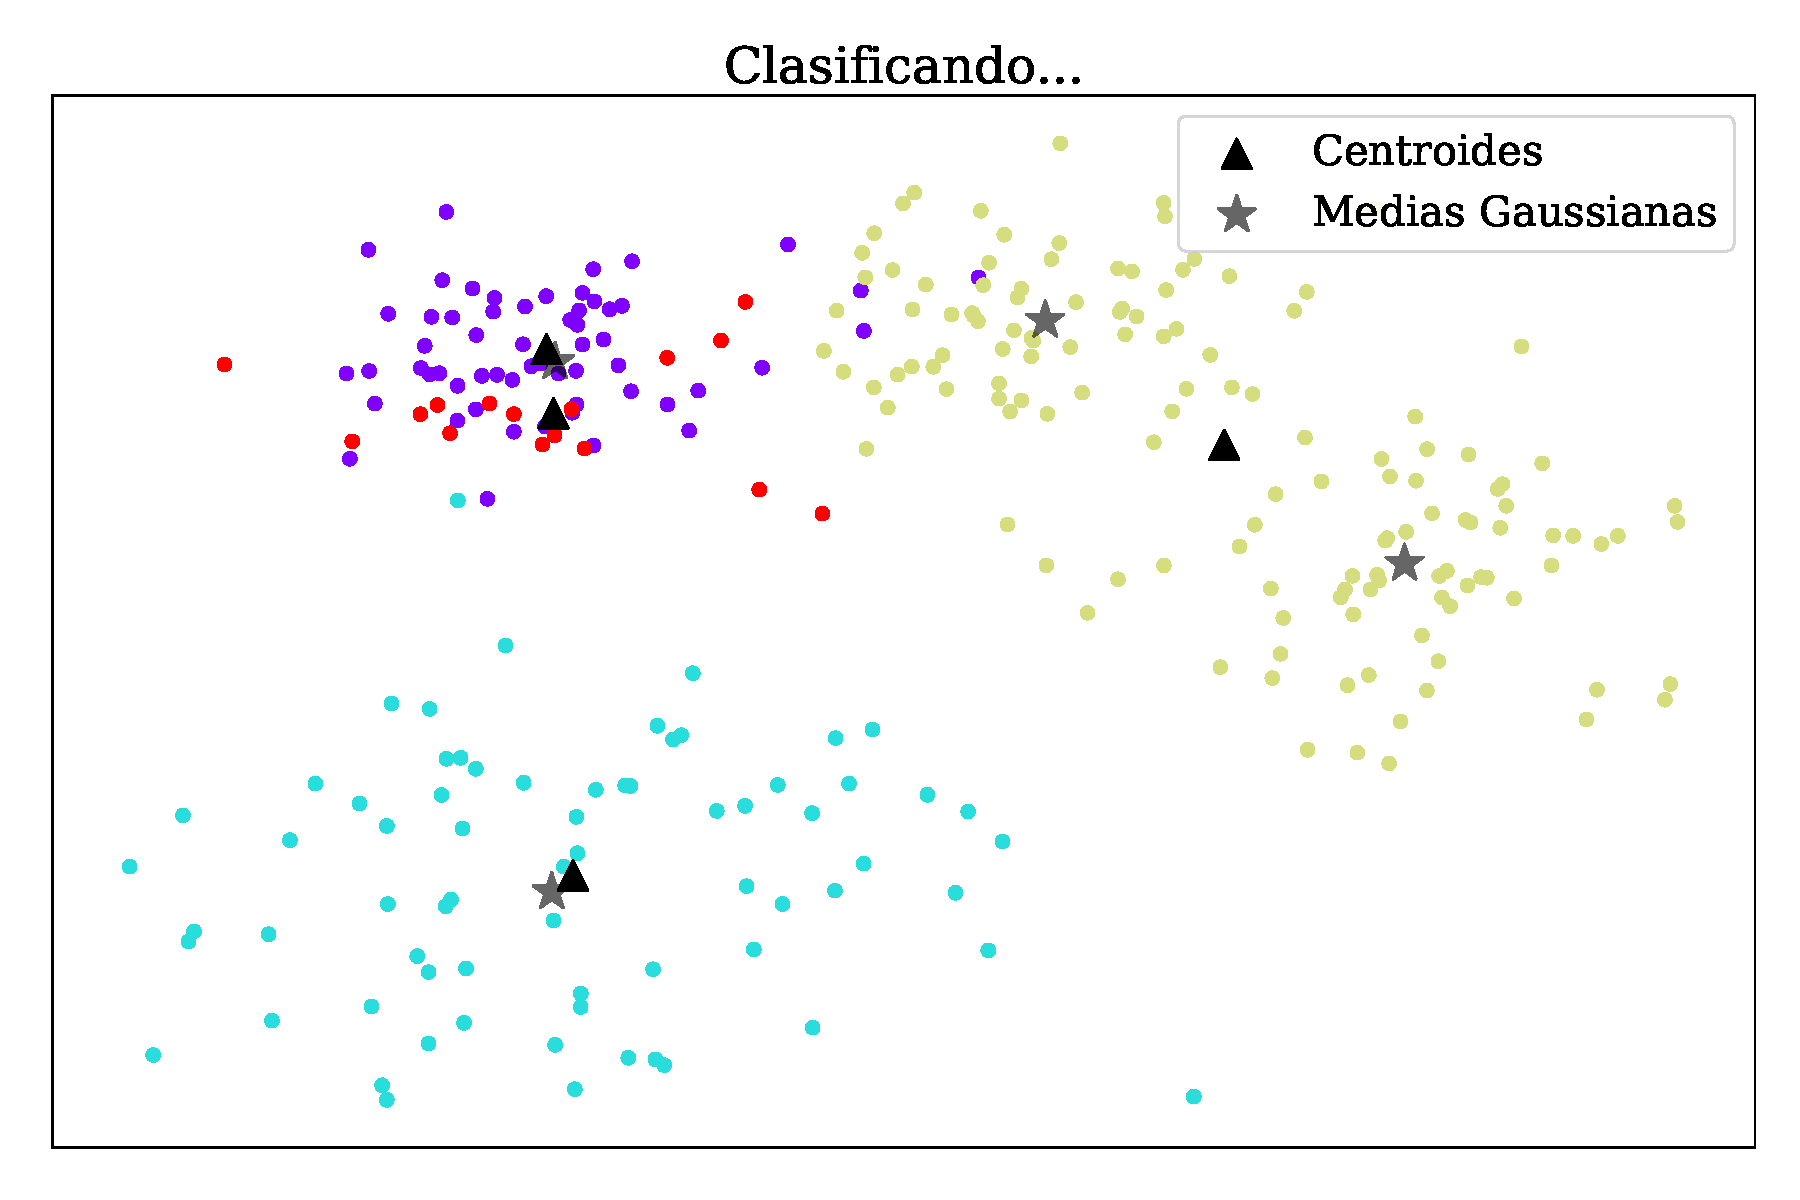
\includegraphics[width=0.475\textwidth]{plots/ejer_2_clasificando_a_conv.pdf}
        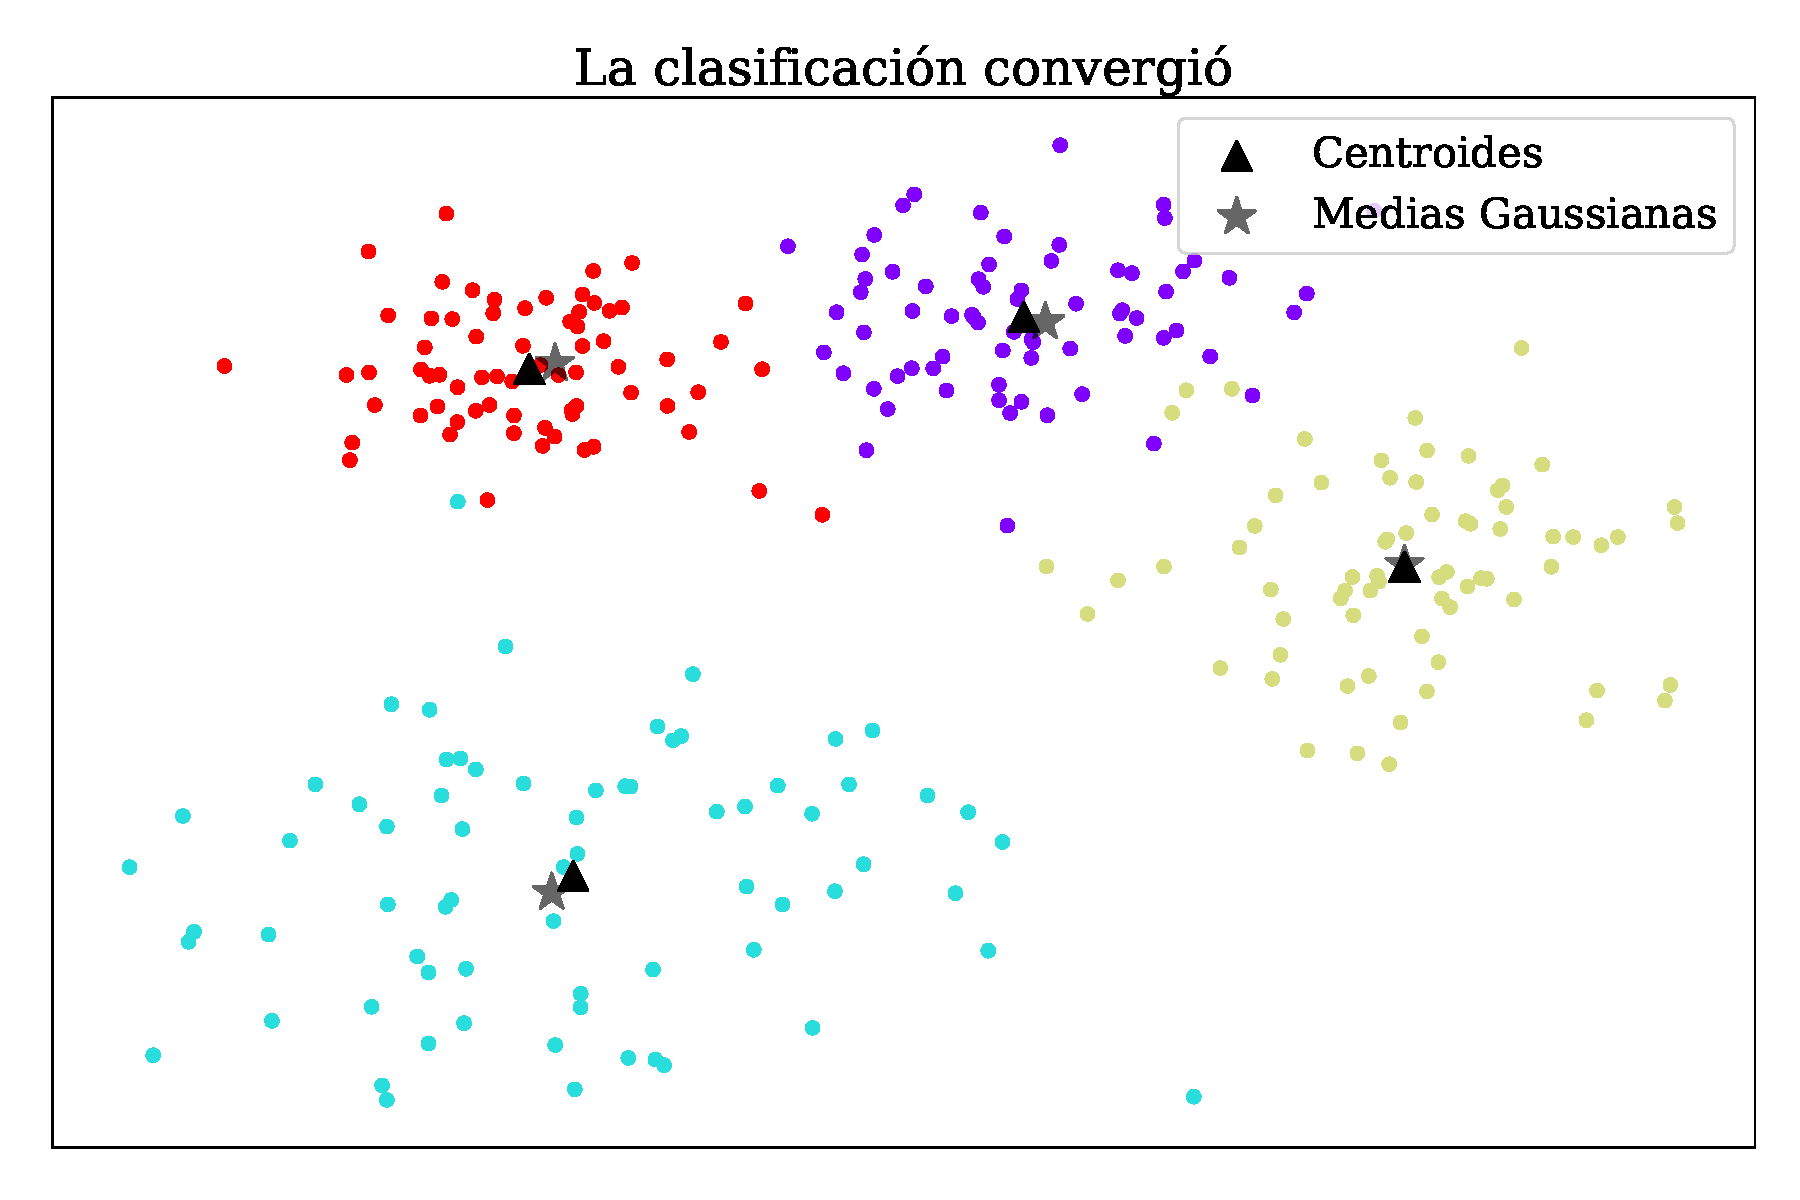
\includegraphics[width=0.475\textwidth]{plots/ejer_2_si_converge.pdf}
        \caption{Estados inicial y final de la clasificación  del \emph{k-means}. La figura superior muestra los valores iniciales de los centroides y la clasificación inicial de los puntos. En la figura inferior se observa que la clasificación convergió y los centroides convergen a puntos cercanos a las medias de las gaussianas  usadas para generar los puntos.}
        \label{fig:ejer2_converge}
    \end{figure}

    En la figura \ref{fig:ejer2_no_converge} se observa un ejemplo de cuando el algoritmo no converge a una solución coherente con el conjunto de datos generado. %Este es un ejemplo donde no funciona

    \begin{figure}[H]
        \centering
        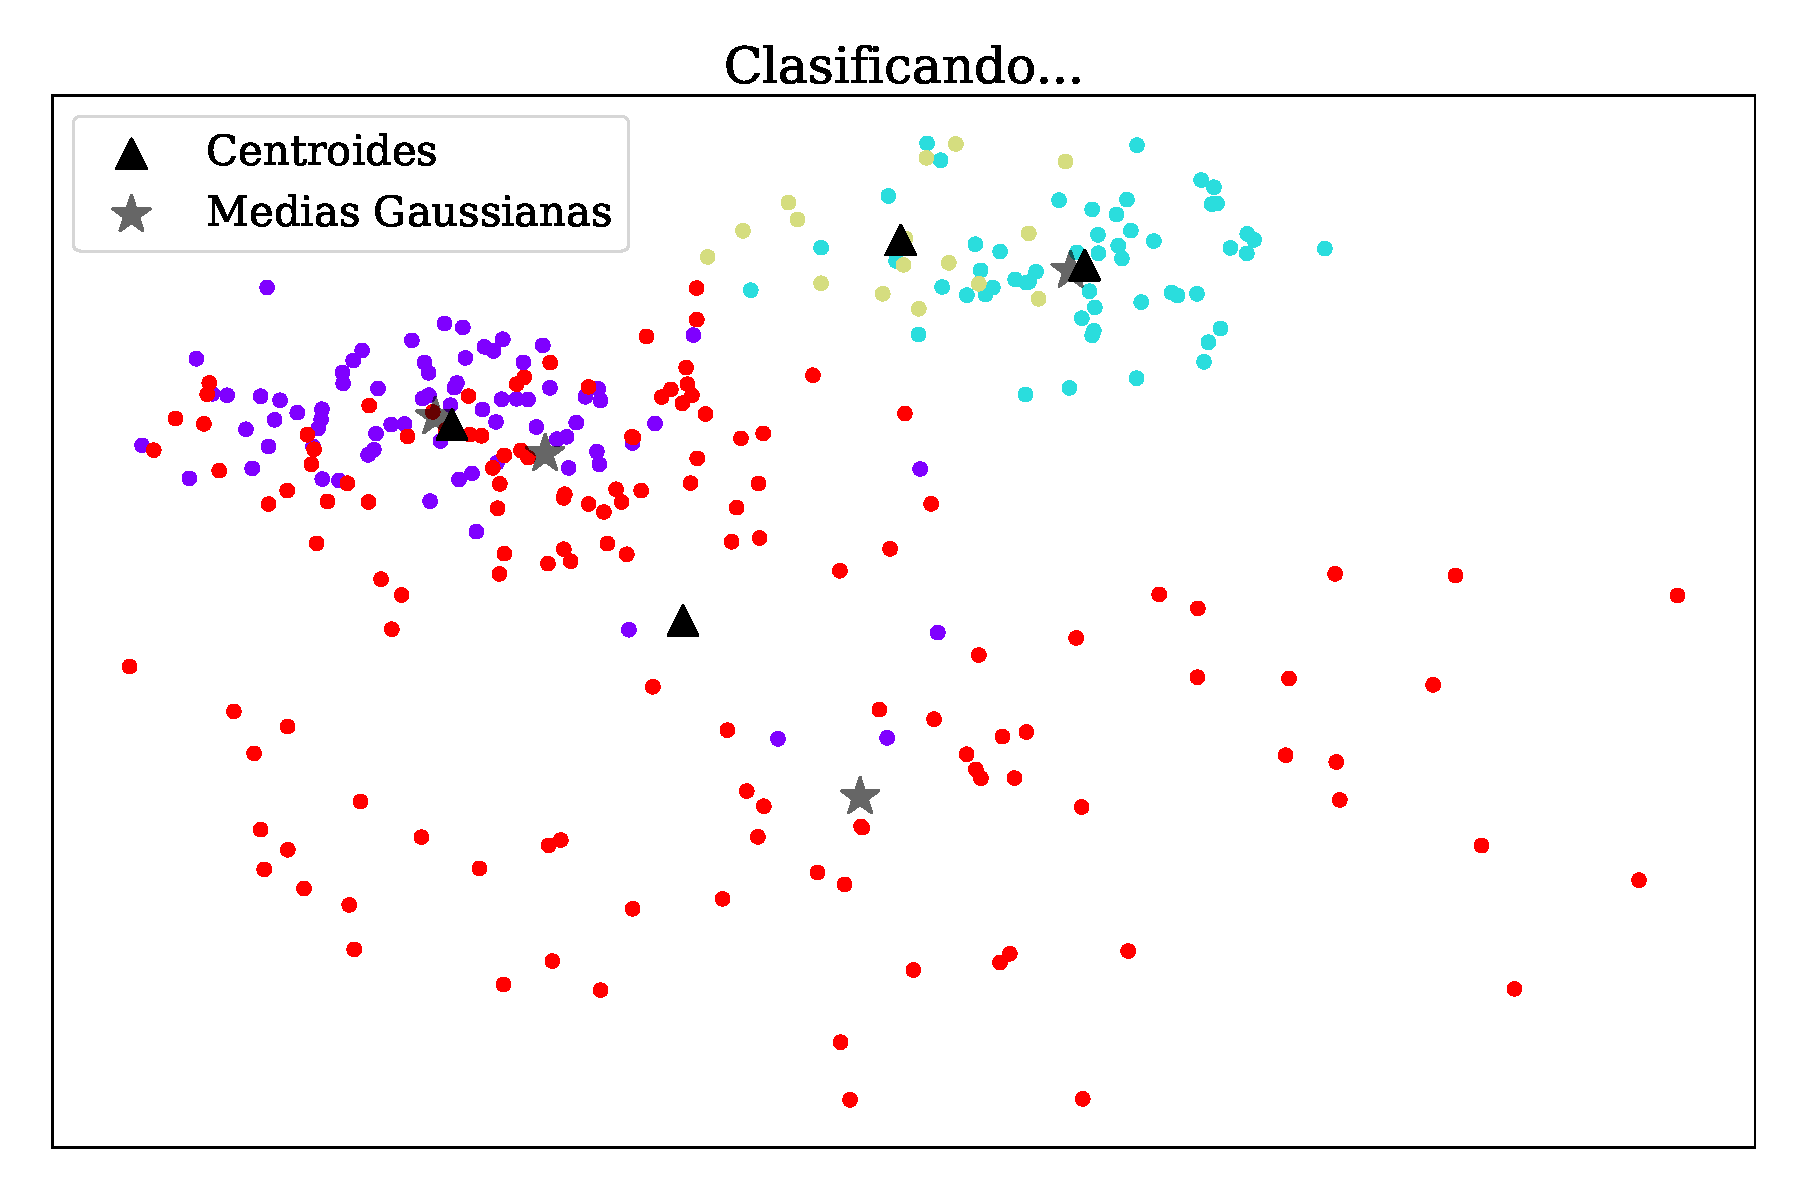
\includegraphics[width=0.5\textwidth]{plots/ejer_2_clasificando.pdf}
        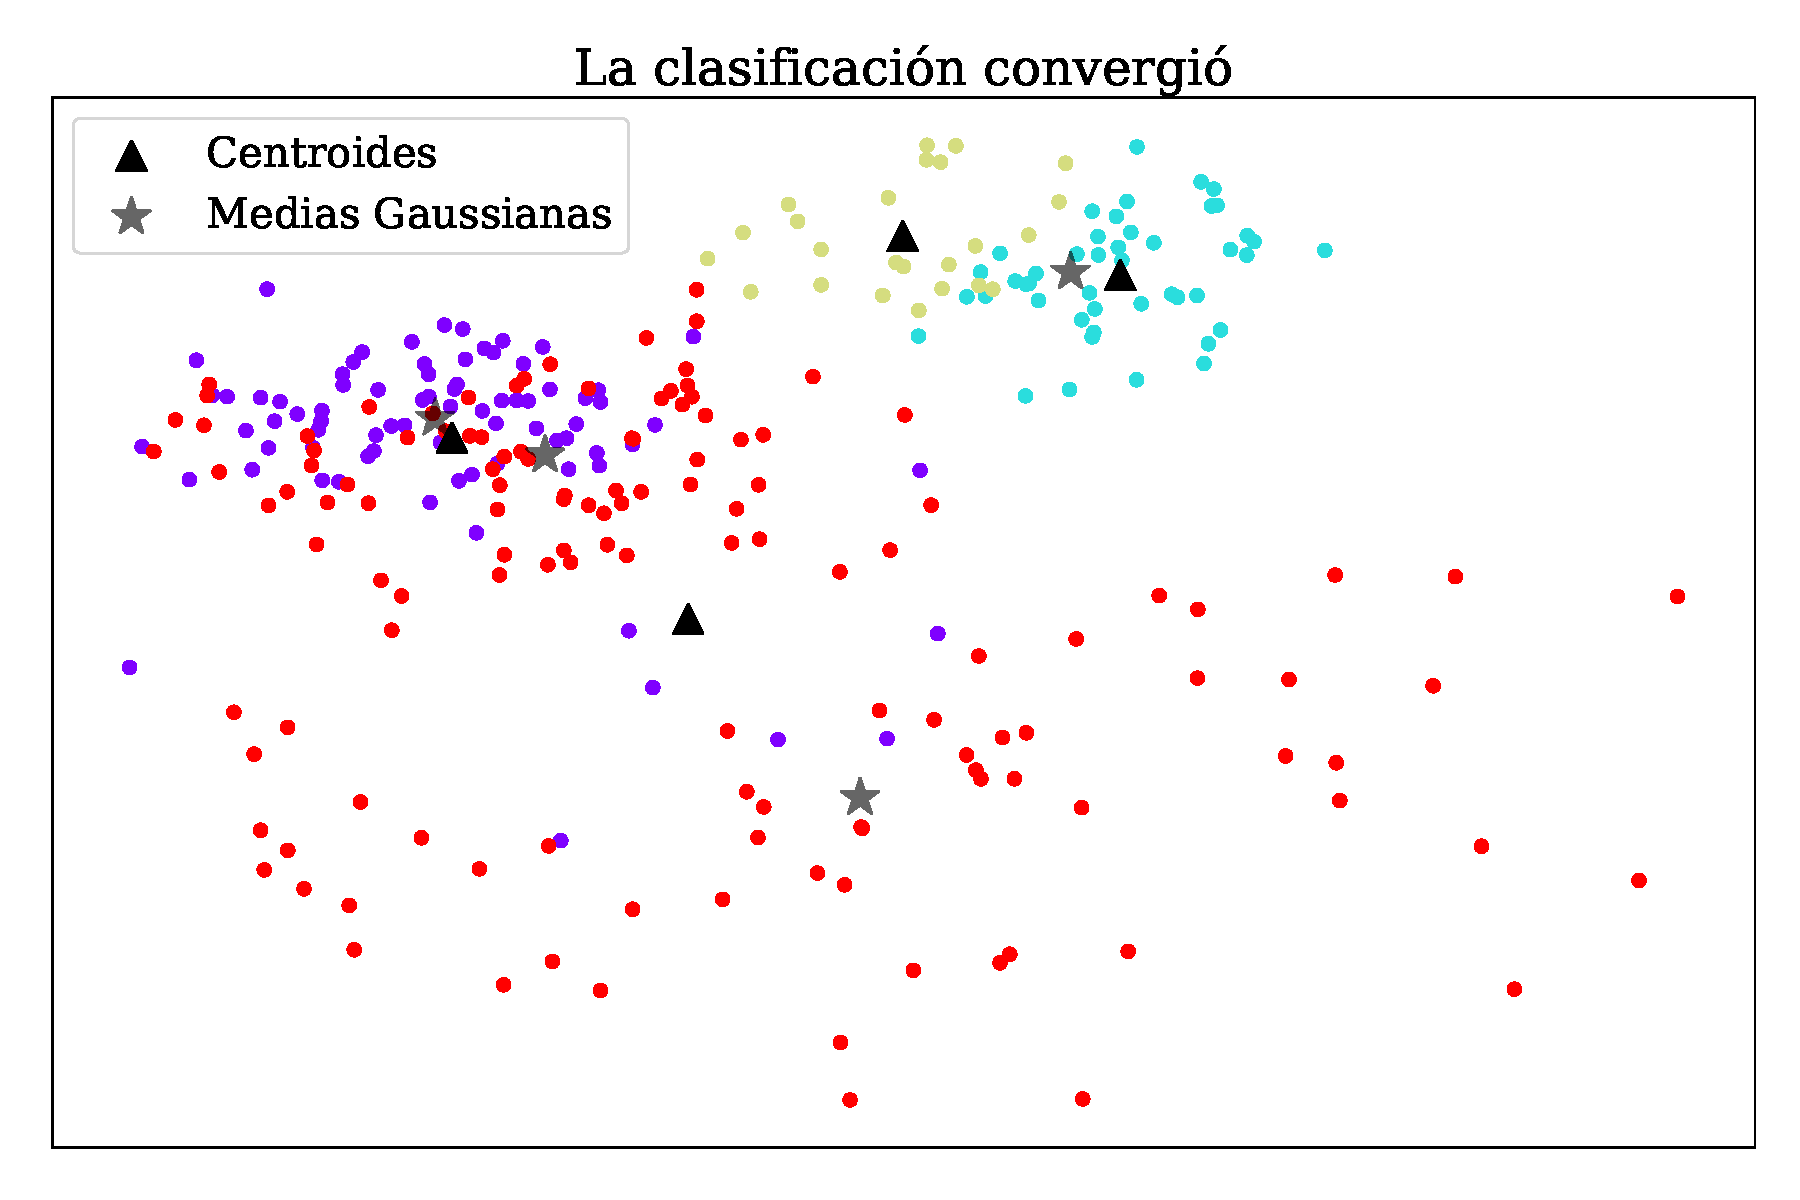
\includegraphics[width=0.5\textwidth]{plots/ejer_2_no_converge.pdf}
        \caption{Estados inicial y final de la clasificación  del \emph{k-means}. En esta ejecución del programa, los centroides no convergen a las medias y en general la clasificación  es pobre.}
        \label{fig:ejer2_no_converge}
    \end{figure}

   \section*{Ejercicio 3}

   Para este ejercicio se utilizó el módulo \verb|datasets| de la librería \verb|Keras| para cargar los datos de entrenamiento y validación del MNIST y CIFAR-10, para utilizar el algoritmo de \emph{KNN} para la clasificación.

   La ejecución del programa se imprime lo siguiente  en la salida estándar:

   \begin{verbatim}
Con el MNIST: 
Dimensiones del set de entrenamiento:  
(60000, 28, 28)

60000 ejemplos de entrenamiento
10000 ejemplos para probar

100.0% probando con 20 ejemplos


Con el CIFAR-10: 
Dimensiones del set de entrenamiento:
(50000, 32, 32, 3)

50000 ejemplos de entrenamiento
10000 ejemplos para probar

30.0% probando con 20 ejemplos
   \end{verbatim}


    \section*{Ejercicio 4}

    Usando los datos generado para el ejercicio  2 como datos de entrenamiento  y  validación y se implementó el algoritmo \emph{KNN} para clasificar $375$ puntos,   distribuidos en  5 distribuciones normales  con media y dispersión aleatorias, en dos dimensiones para 1, 3 y 7 vecinos. 

    %\subsection*{Número de vecinos $k=1$}

    Dependiendo de la clasificación de \emph{k-means}, el algoritmo de \emph{KNN} puede funcionar o no. En el caso presentado en la Fig.\,\ref{fig:ejer4_k_1_malo} se observa que el \emph{k-means} separó a los conjuntos de datos coherentemente pero el algoritmo de \emph{KNN} convergió a  una solución errónea, se presentaron $125$ ejemplos de validación de los cuales el $36\%$ fueron clasificados correctamente.

    \begin{figure}[H]
    \centering
    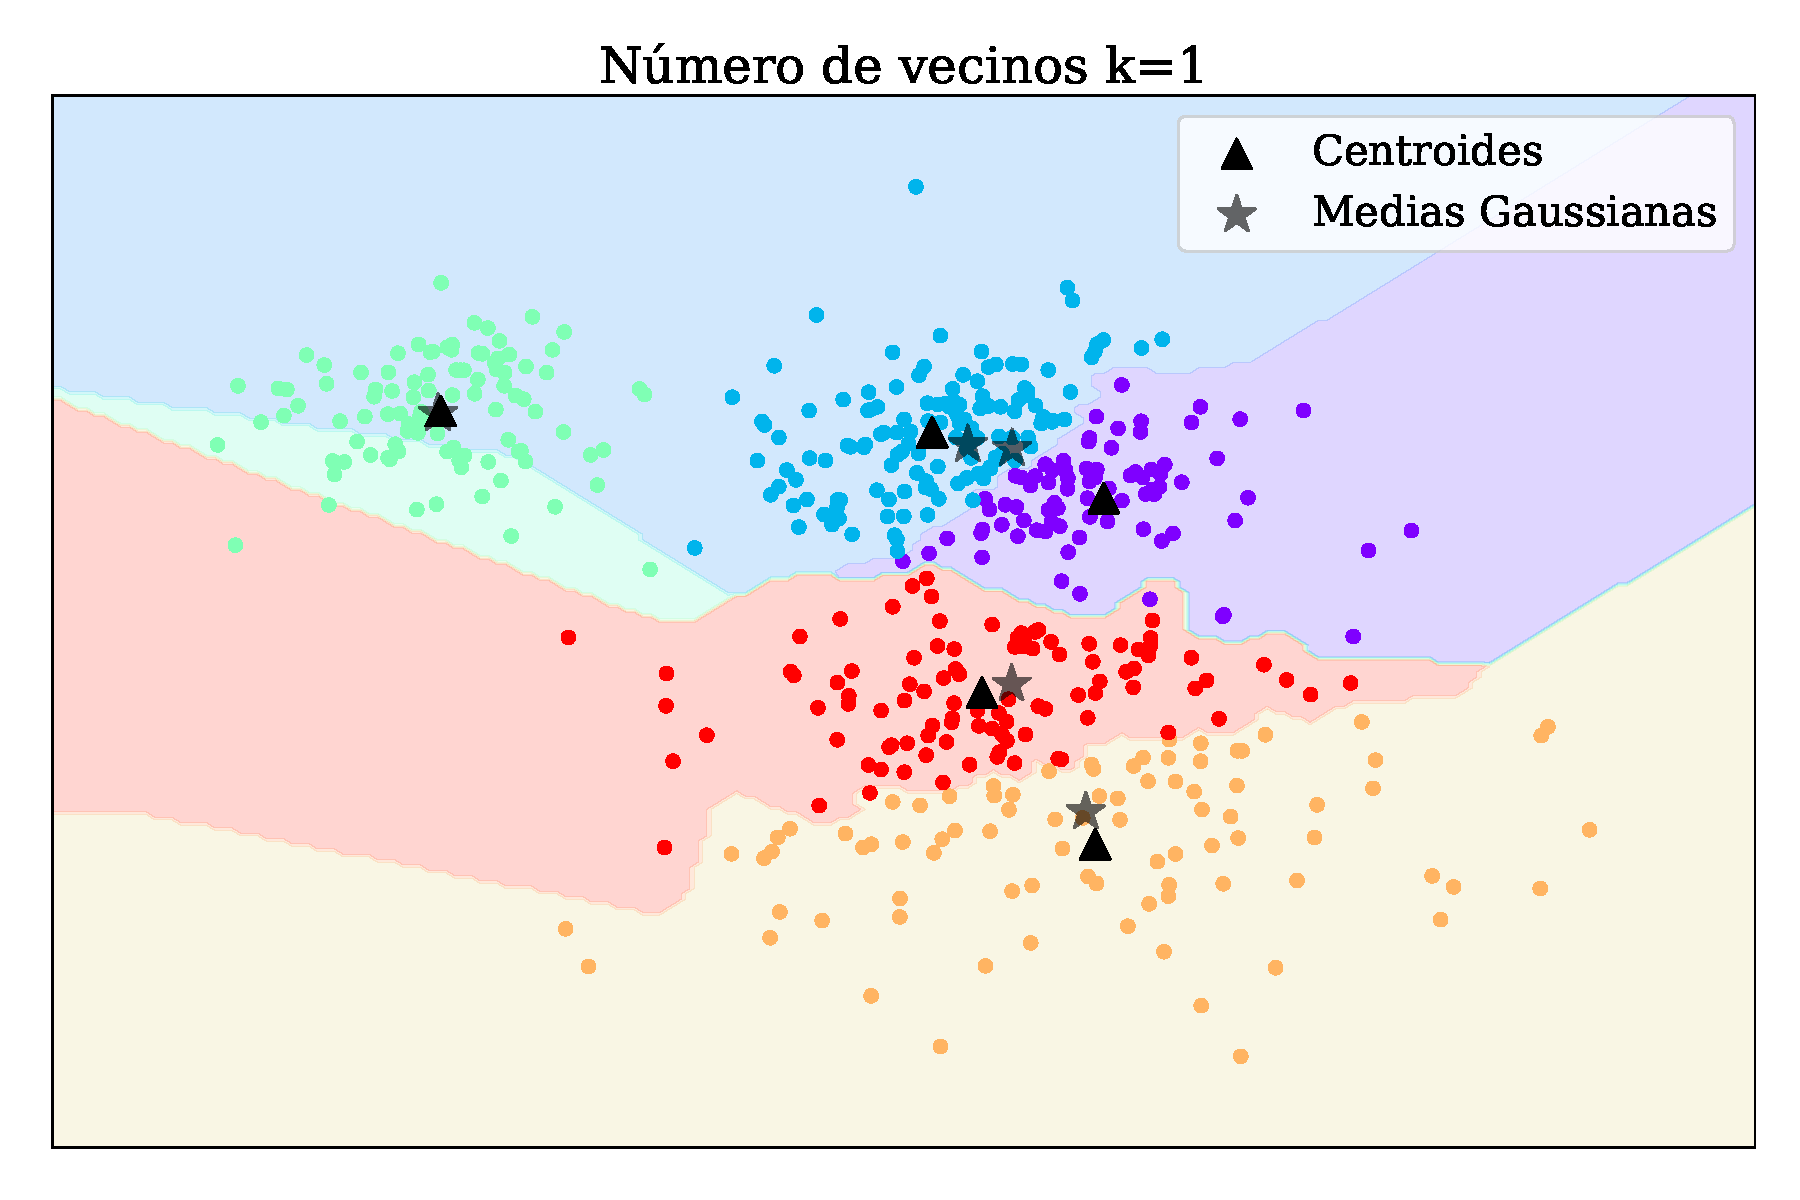
\includegraphics[width=0.45\textwidth]{plots/ejer_4_K-1_no_coverge.pdf}
    \caption{Estado final de la clasificación del algoritmo de \emph{KNN} con $K=1$, en la validación con 125 datos solo se pudo calificar correctamente el 36.0\%.}
    \label{fig:ejer4_k_1_malo}
    \end{figure}

    En la Fig.\ref{fig:ejer4_k_1} se observa que el algoritmo converge a una solución, dando $99.2$ de aciertos en los 125 ejemplos de validación.

    %\subsection*{Número de vecinos $k=3$}

    Para una cantidad de vecinos $k=3$, las  simulaciones y clasificaciones en promedio daban un porcentaje de aciertos menor que $k=1$. En el caso de la Fig.\,\ref{fig:ejer4_k_3} se obtuvo un $94.4\%$ probando con 125 ejemplos. 

        %\subsection*{Número de vecinos $k=7$}

    Para una cantidad de vecinos $k=7$, el rendimiento de las  simulaciones y clasificaciones en promedio eran peor que los casos anterior. En el caso de la Fig.\,\ref{fig:ejer4_k_7} se obtuvo un $72.0\%$ probando con 125 ejemplos. Para $k=7$, la solución a la que converge el algoritmo no tiene la misma generalización que para $k=1$ y $k=3$.


\begin{figure}[H]
    \centering
    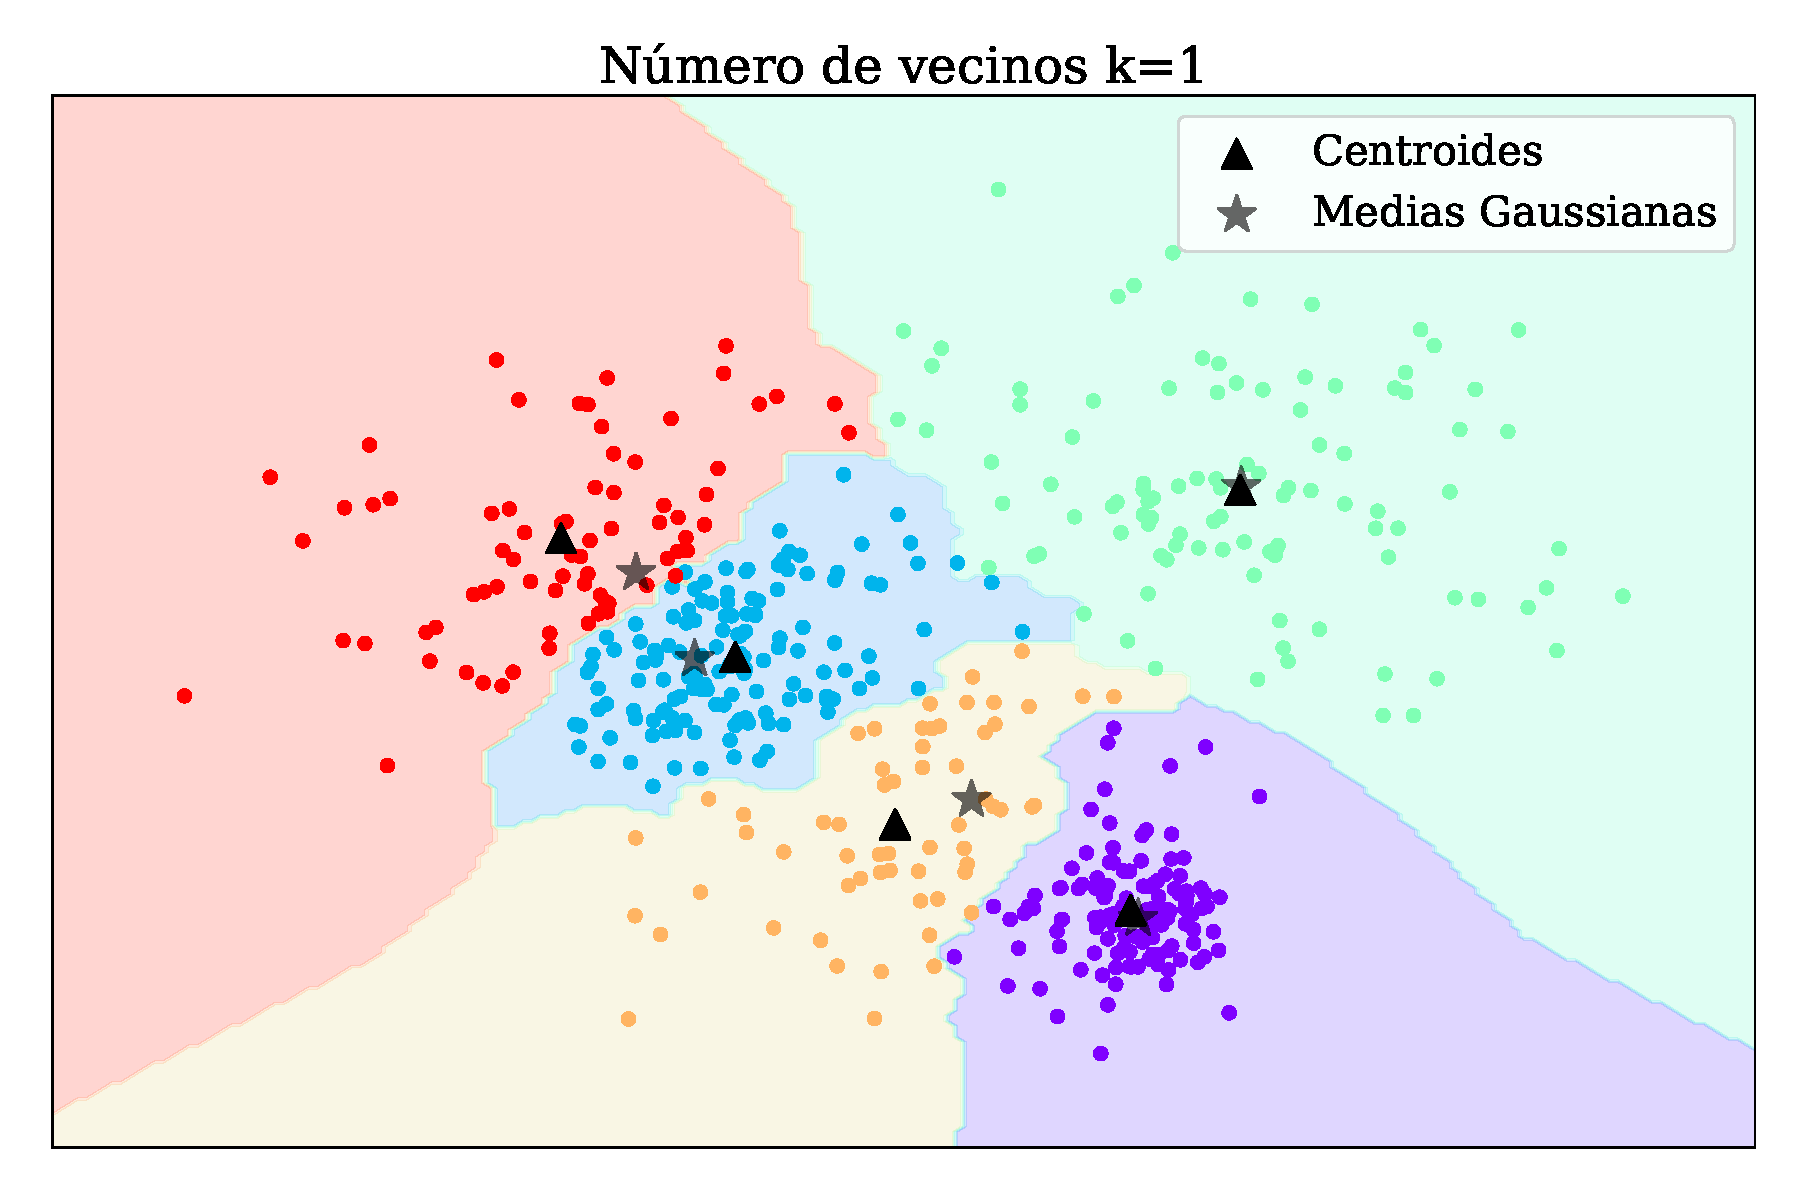
\includegraphics[width=0.45\textwidth]{plots/ejer_4_K-1_si_converge.pdf}
    \caption{Estado final con $K=1$. Se observa que la clasificación se corresponde con el entrenamiento y en la validación se obtuve un $99.2\%$ de acierto con 125 datos.}
    \label{fig:ejer4_k_1}
\end{figure} 

\begin{figure}[H]
    \centering
    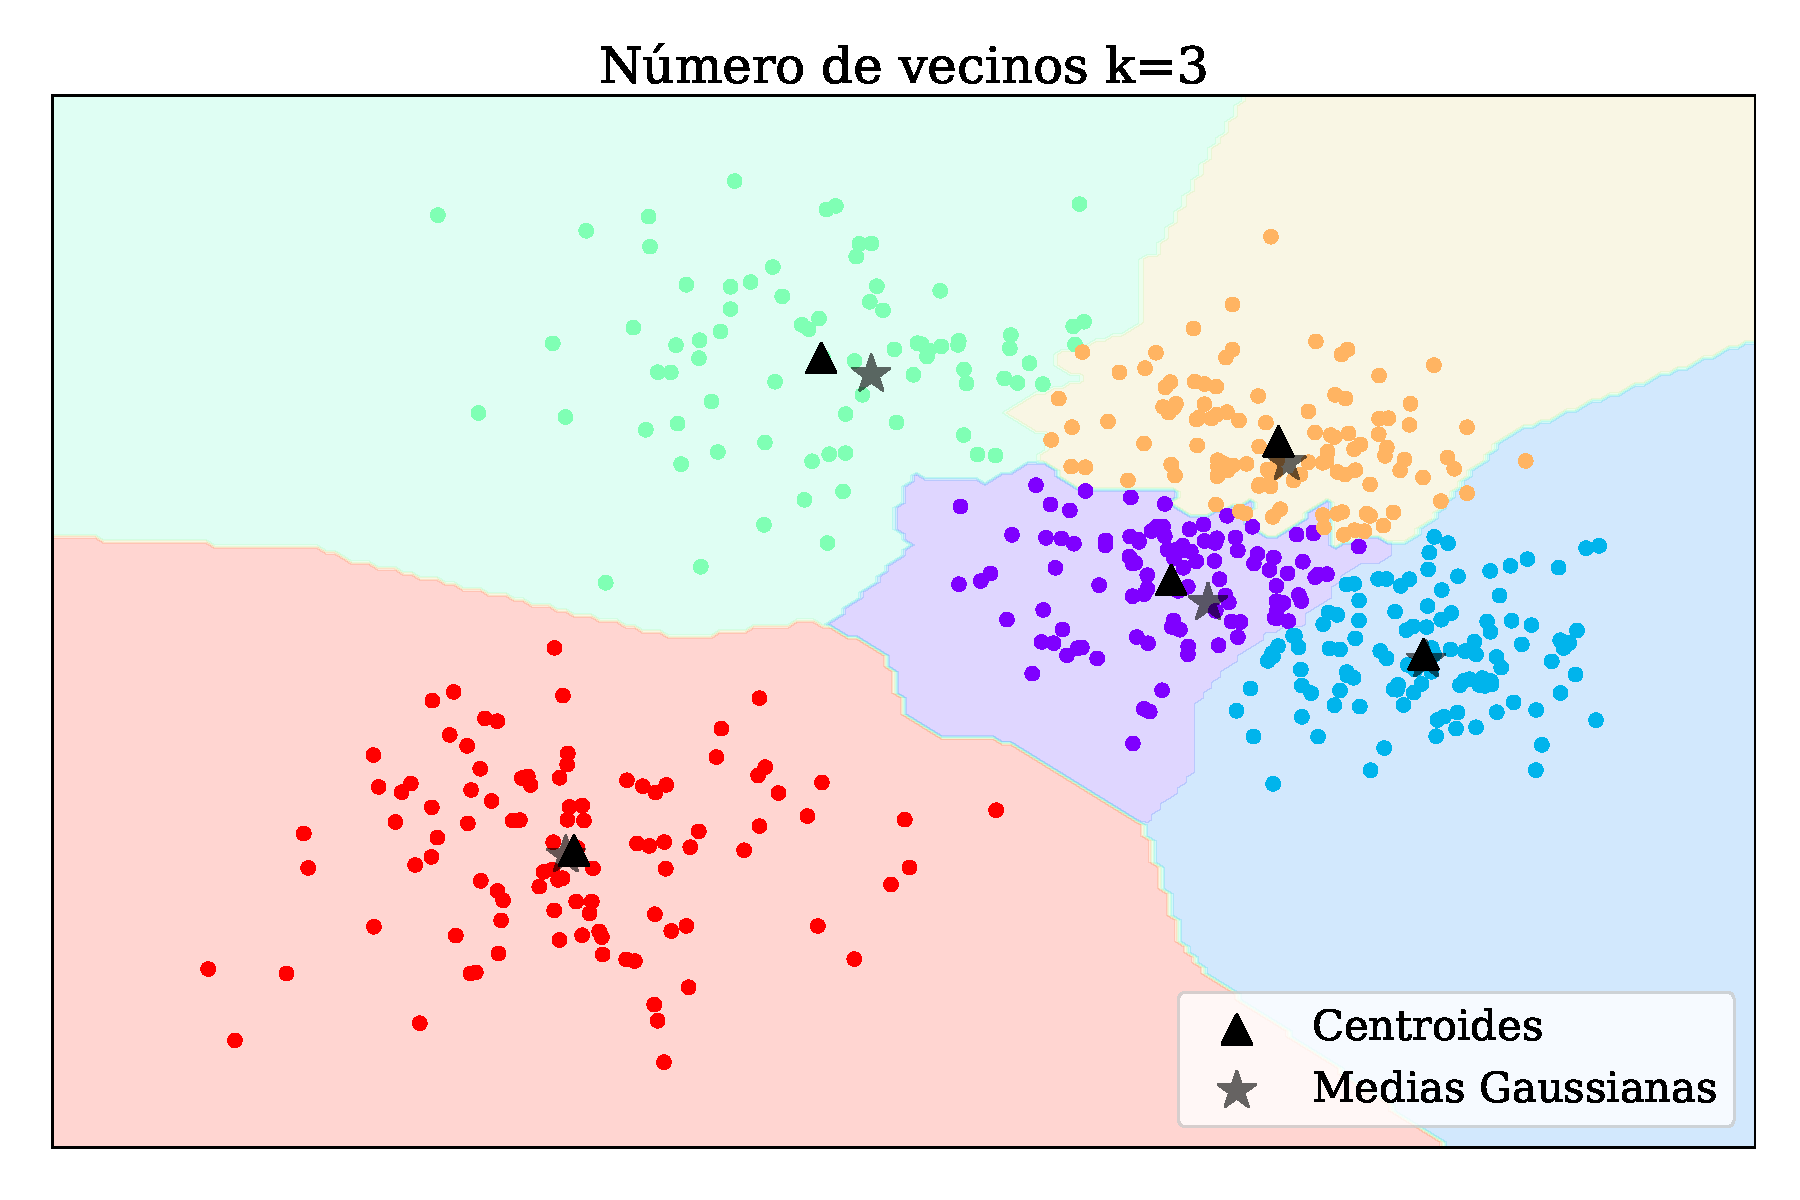
\includegraphics[width=0.45\textwidth]{plots/ejer_4_K-3_si_converge.pdf}
    \caption{Estado final con $k=3$. Se observa que la clasificación se corresponde con el entrenamiento y en la validación se obtuve un $99.2\%$ de acierto con 125 datos.}
    \label{fig:ejer4_k_3}
\end{figure} 

\begin{figure}[H]
    \centering
    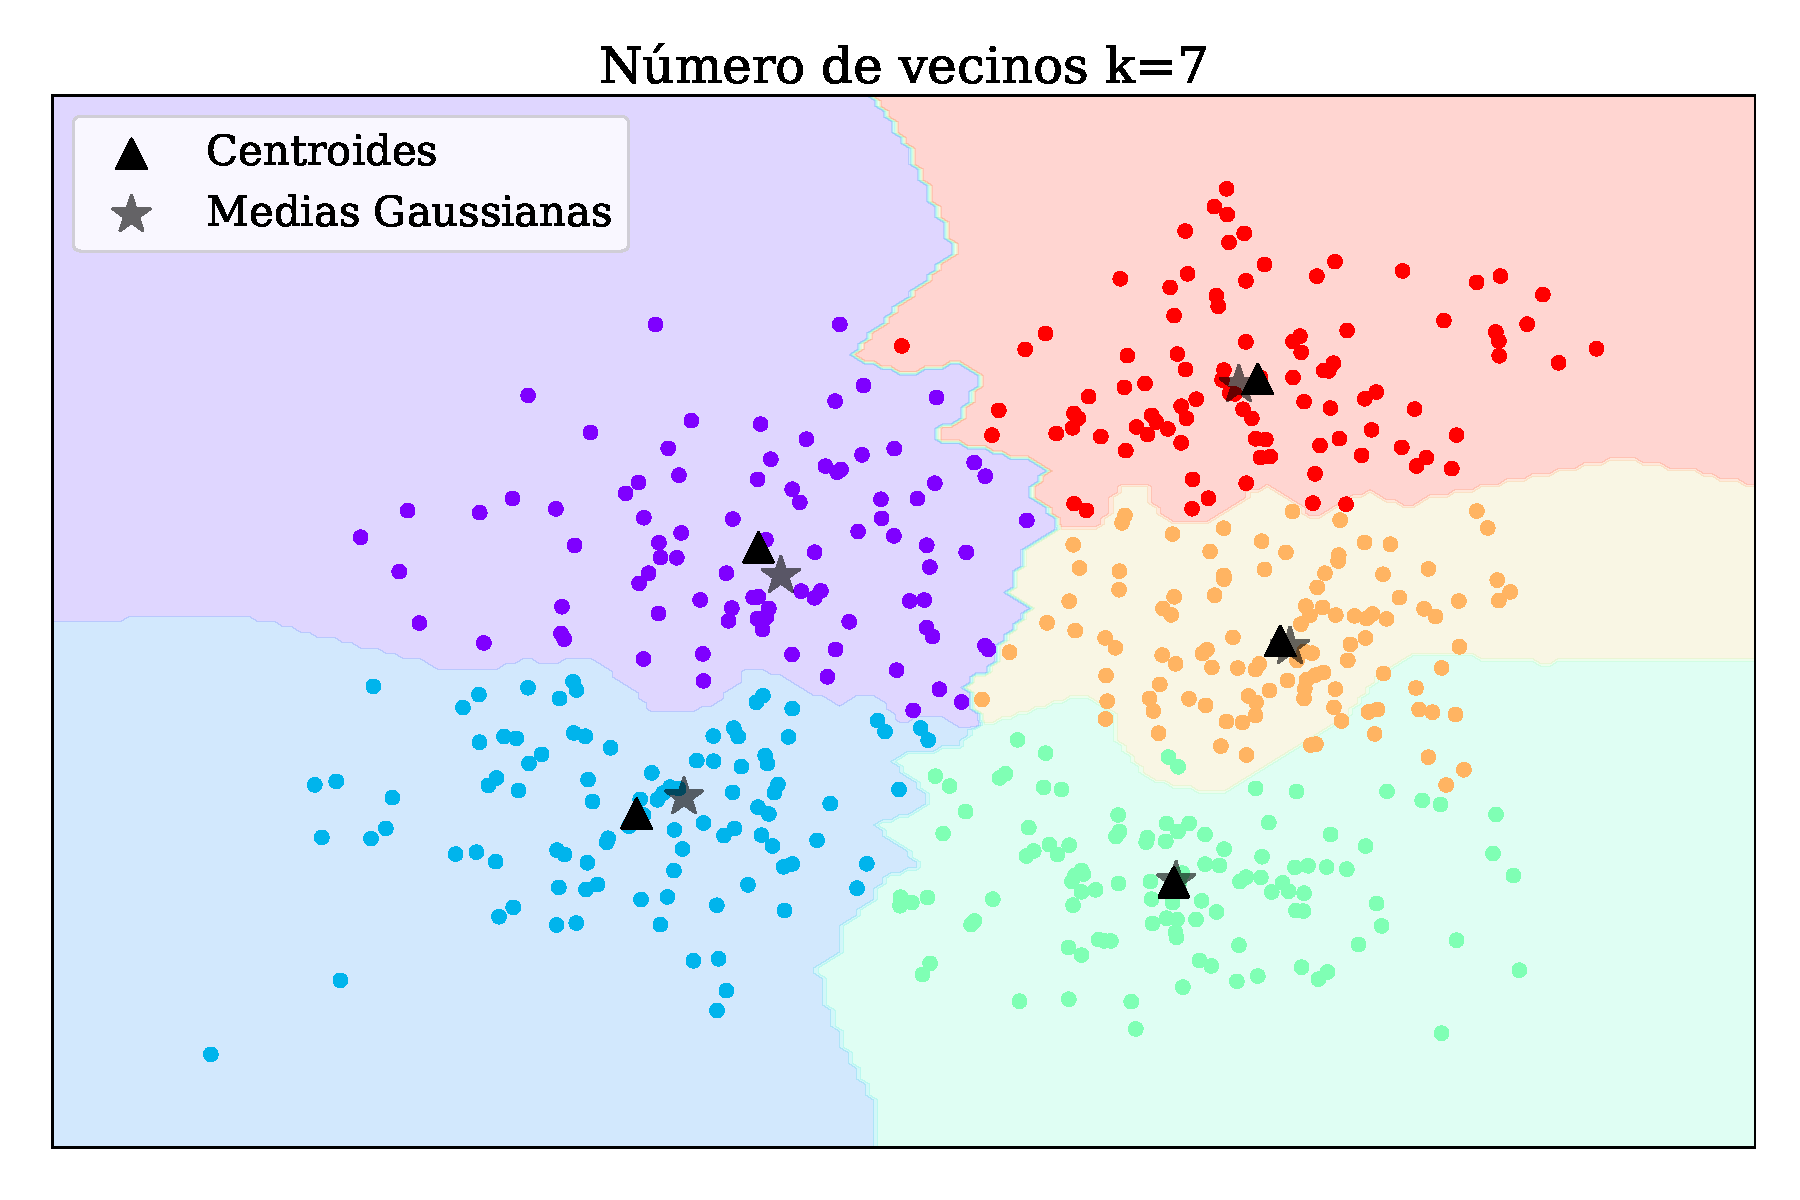
\includegraphics[width=0.45\textwidth]{plots/ejer_4_K-7_si_converge.pdf}
    \caption{Estado final con $k=7$. El algoritmo pierde generalización y en la validación se obtiene un $72.0\%$ de acierto con 125 datos. }
    \label{fig:ejer4_k_7}
\end{figure} 
    

\section*{Ejercicio 5}

En este ejercicio se implementaron los clasificadores lineales \emph{Support Vector Machine} y \emph{SoftMax} para clasificación de los conjuntos de datos del \emph{MNIST} y \emph{CIFAR-10}, almacenados en el módulo \verb|datasets| de la librería \verb|keras|.  módulo ya proporciona los datos de entrenamiento y validación para ambos casos. En la función de pérdida se agregó una función de regularización del tipo $L_2$.

Si implementó la clase \verb|LinearClassifier| donde se definieron las funciones de:
\begin{itemize}
    \item Inicialización:

    En la inicialización se definen los parámetros de tasa de aprendizaje  $\eta$, la cantidad de épocas \verb|epochs|, el parámetro de la normalización $\lambda_{L2}$, el tamaño del batch de datos  para el \emph{gradiente estocástico por batch}, y también se  define si se implementa el uso de bias o no.

    \item  \verb|fit|:

    Esta función recibe el conjunto de datos de entrenamiento y validación. Transforma las imágenes en vector unidimensionales, dependiendo si utiliza el bias, se agregan el uno al inicio de cada imagen.

    También en esta función se inicializa la matriz  de peso de forma uniforme entre $[-0.1, 0.1]$, como también se normaliza a las imágenes con el valor máximo de cada elemento que estas dos bases de datos es $255$.

    Esta función recorre el conjunto de datos durante la cantidad de épocas definida en la inicialización. También realiza el entrenamiento por batch y la validación. Los valores de precisión y pérdida por época se almacenan en vectores inicializados en esta función.

    \item \verb|predict|

    Esta función devuelve la clasificación predicha por la matriz de pesos dada un época.

    \item \verb|loss_gradient|

    Esta función es propia de cada método de clasificación lineal. En la definición de las subclases \verb|SVM| y \verb|SMC| se detallan la funciones de pérdida y el gradiente de la matriz de pesos.
\end{itemize}

La precisión y la pérdida en función para los datos son calculados con las siguientes parámetros:

\begin{table}[H]
    \centering
    \begin{tabular}{c|c|c|c|c|c}
             &  $\eta$ & Épocas & Batch & $\lambda_{L2}$ & Bias \\ \hline
    MNIST    &  0.0001 & 200 & 32 & 0.1 & Sí \\ \hline
    CIFAR-10 &  0.0001 & 200 & 50 & 0.1 & Sí \\ 
    \end{tabular}
\end{table}
Los mismos se utilizaron para ambos clasificadores.

\subsection*{MNIST} 

Las Figs.\,\ref{fig:ejer5_mnist_acc} y \ref{fig:ejer5_mnist_loss} se muestran los valores de precisión y pérdida en función de la época para CIFAR-10.  Los resultados obtenidos dan una precisión $\sim90\%$ para los datos de entrenamiento y validación. Se observa que para esta base de datos el algoritmo \emph{VSM} tiene una mejor precisión y una menor pérdida con respecto a \emph{SoftMax}.

\begin{figure}[H]
    \centering
    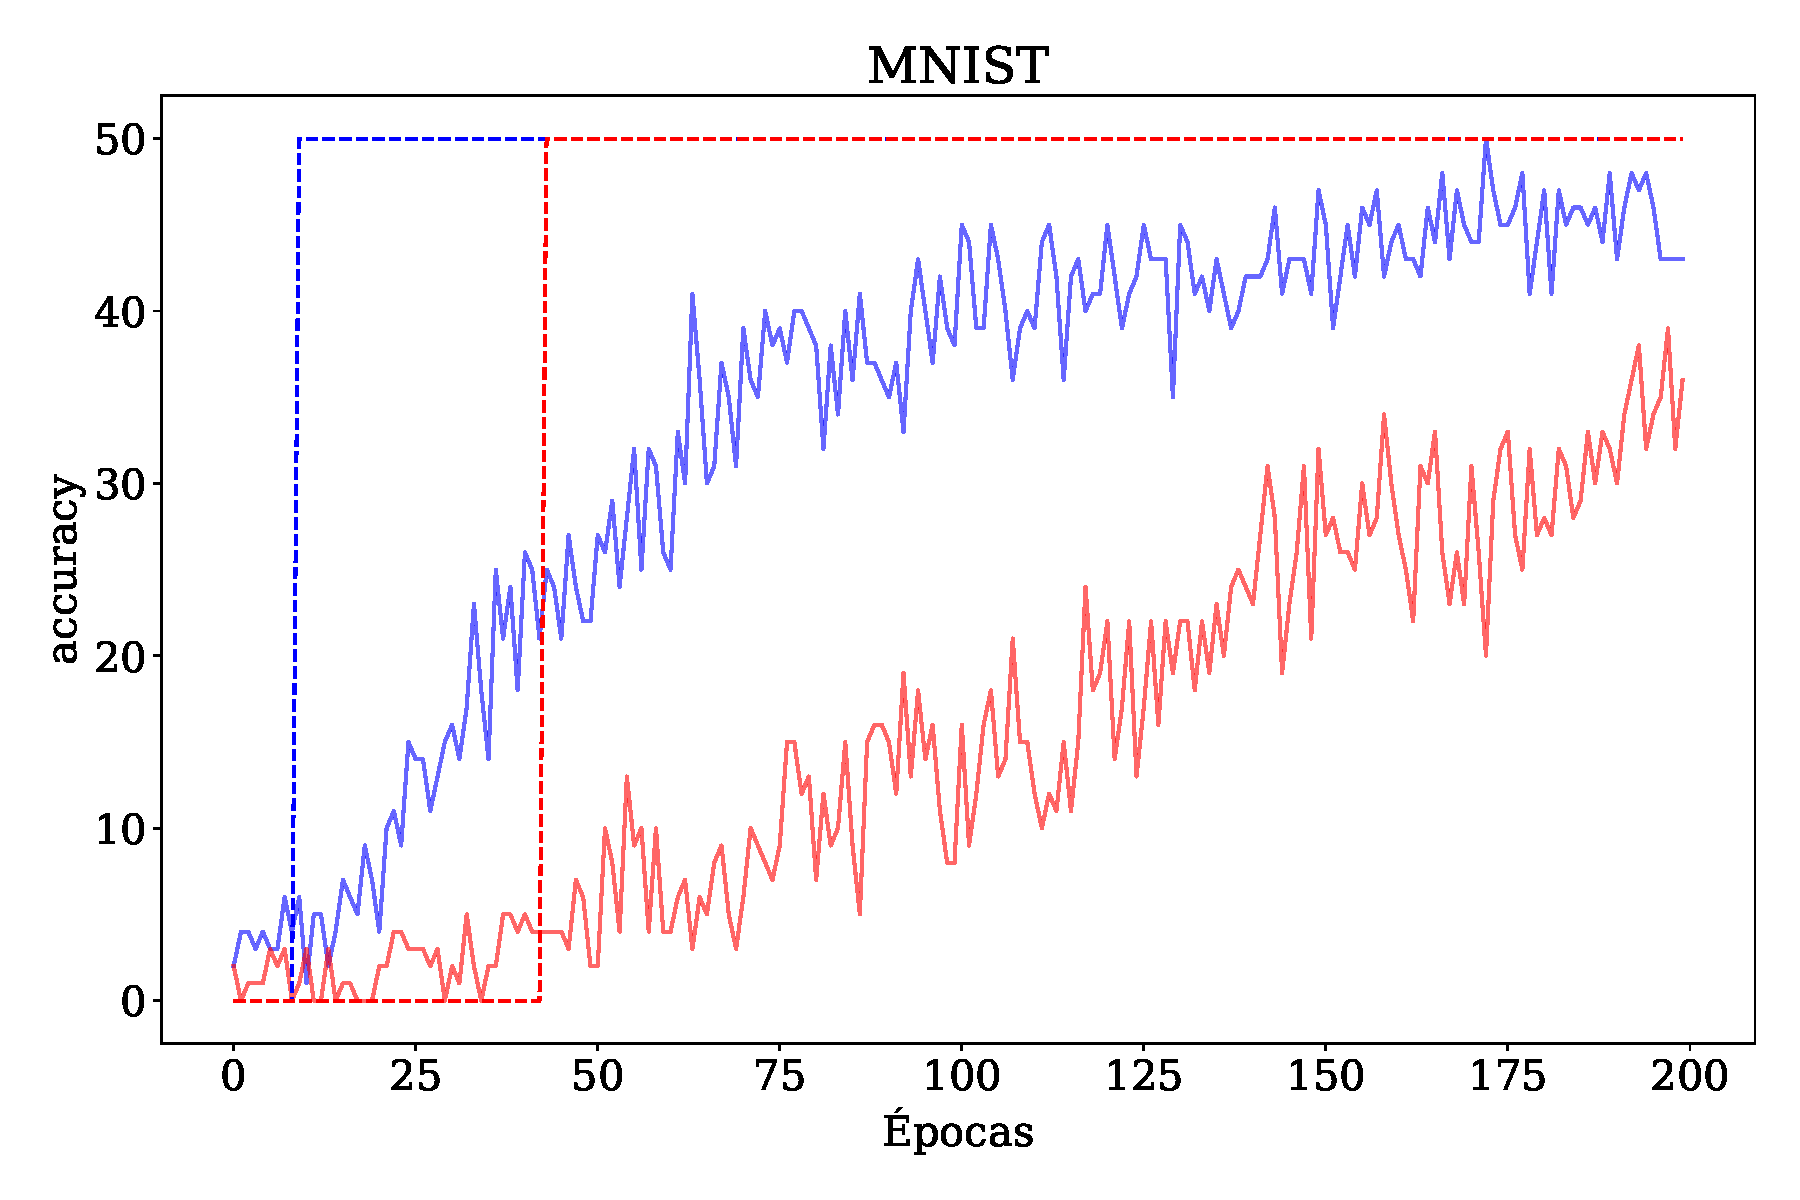
\includegraphics[width=0.5\textwidth]{../../ejer_5_MNIST_acc.pdf}
    \caption{Precisión de los algoritmos sobre el MNIST}
    \label{fig:ejer5_mnist_acc}
\end{figure} 

\begin{figure}[H]
    \centering
    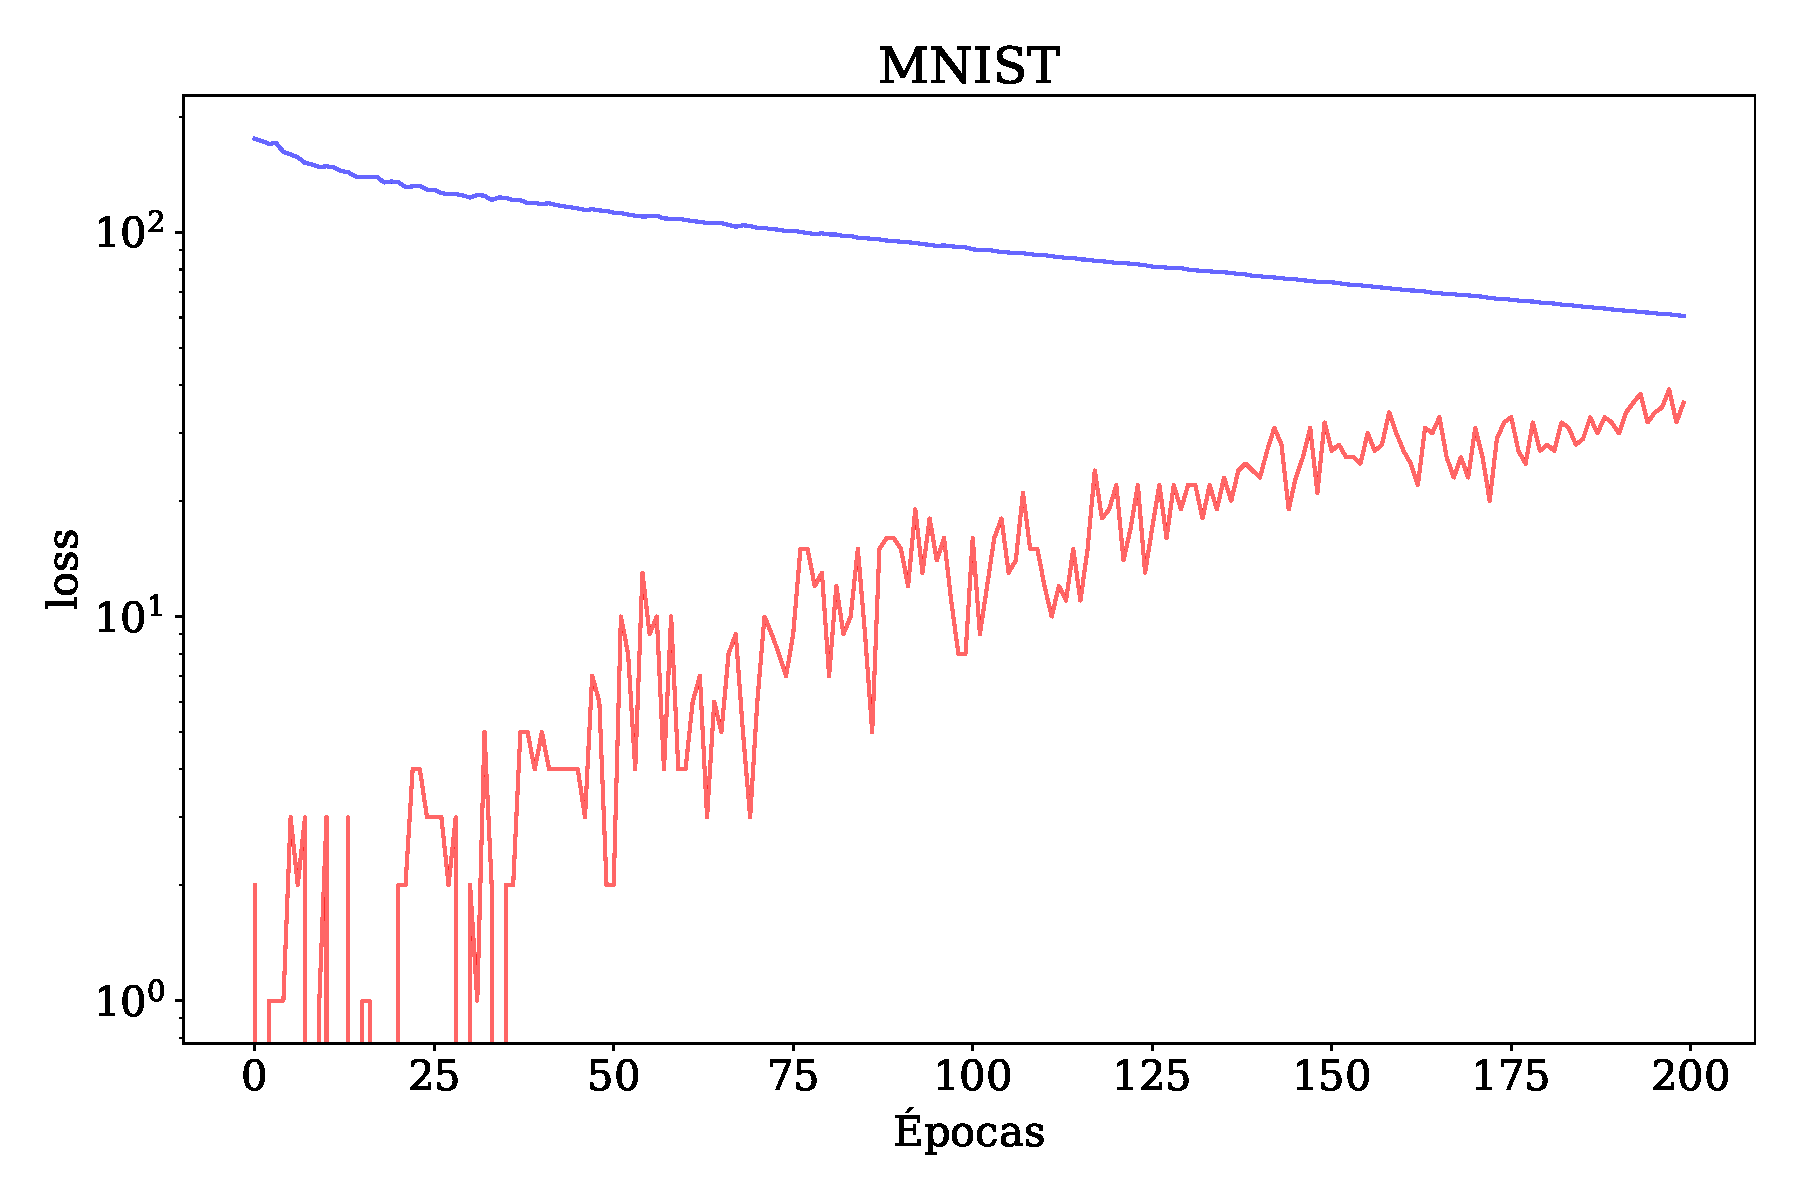
\includegraphics[width=0.5\textwidth]{../../ejer_5_MNIST_los.pdf}
    \caption{Precisión de los algoritmos sobre el MNIST}
    \label{fig:ejer5_mnist_loss}
\end{figure} 


\subsection*{CIFAR-10}

Las Figs.\,\ref{fig:ejer5_cifar10_acc} y \ref{fig:ejer5_cifar10_loss} se muestran los valores de precisión y pérdida en función de la época para CIFAR-10.  Los resultados obtenidos son cercanos a trabajar con una matriz de pesos aleatoria. La implementación realizada en este trabajo no es adecuada para trabajar con esta base de datos. La precisión de \emph{VSM} parece ser mejor que el SoftMax, pero dados los resultados no se puede hablar de una ventaja  de un clasificador por encima de otro.

\begin{figure}[H]
    \centering
    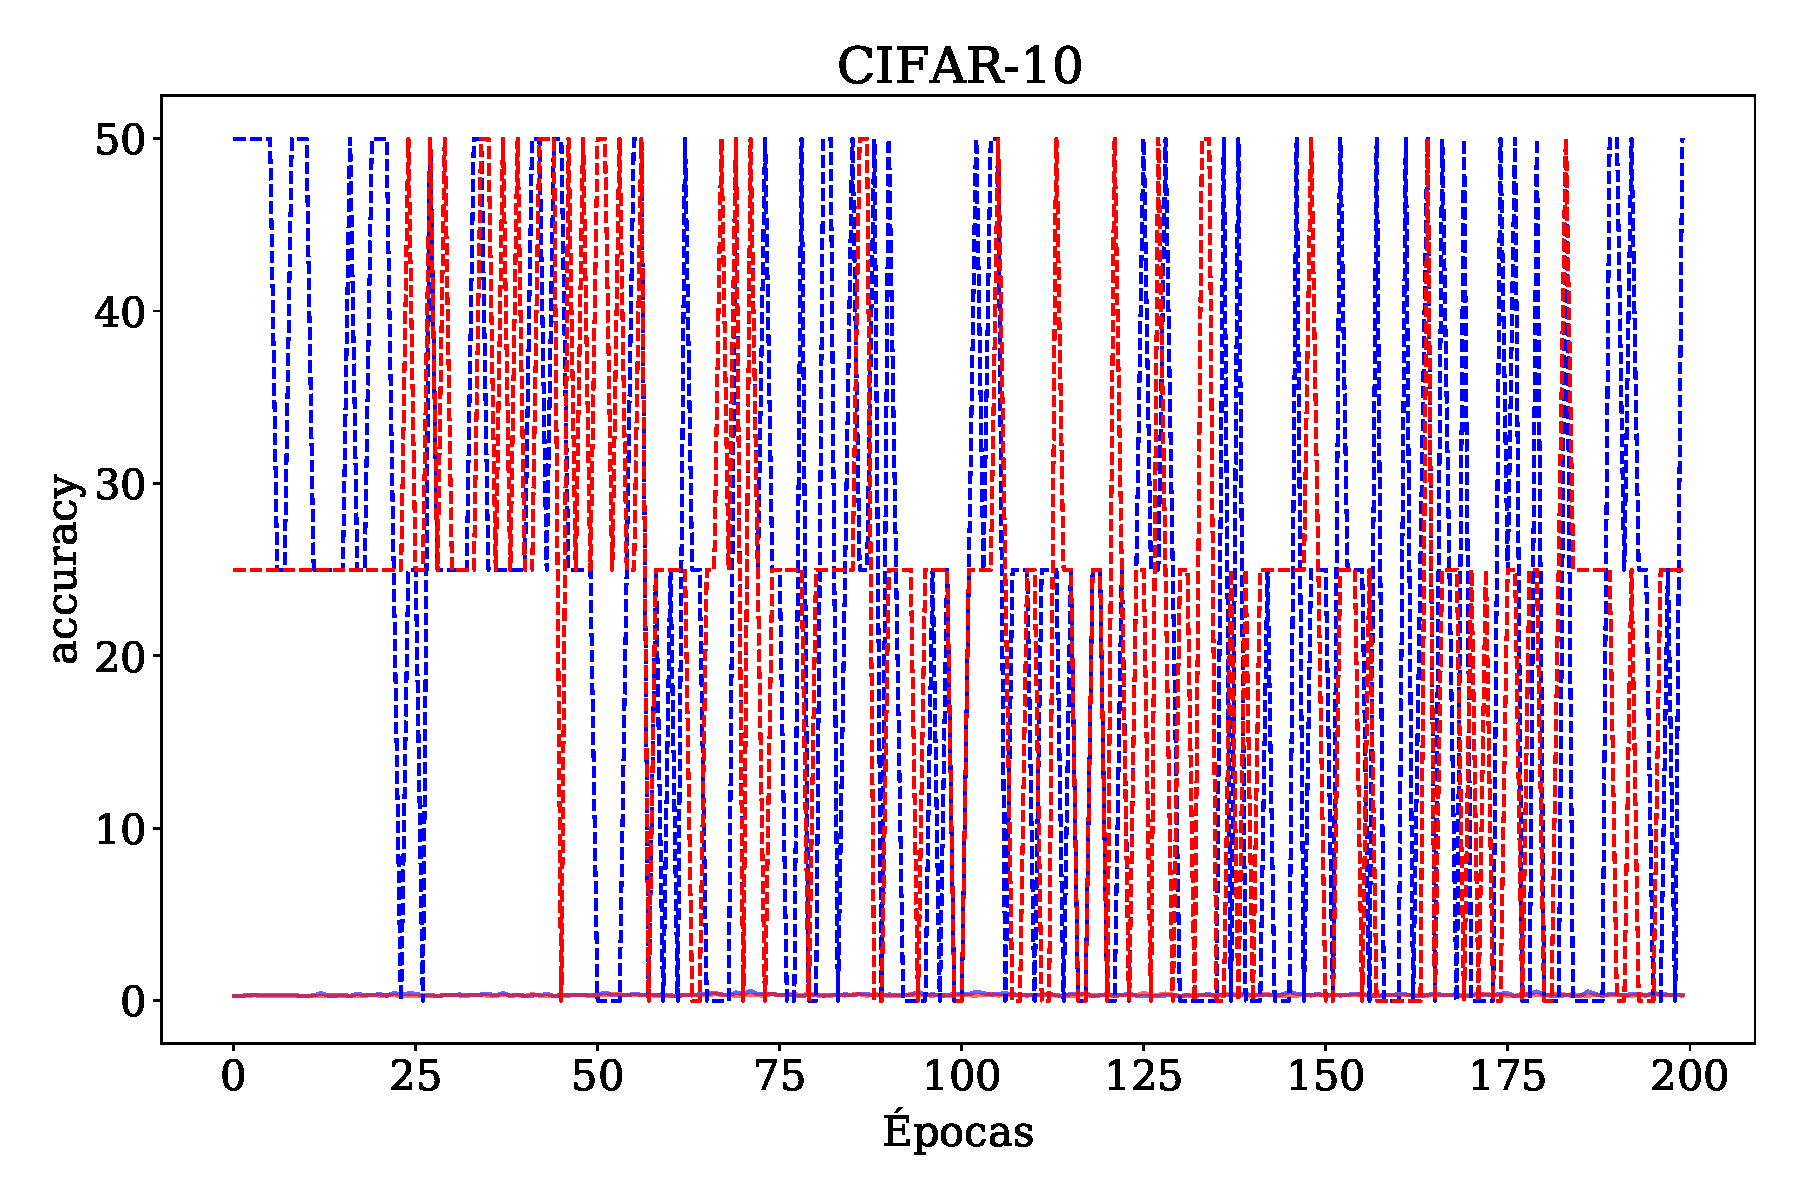
\includegraphics[width=0.5\textwidth]{../../ejer_5_CIFAR-10_acc.pdf}
    \caption{Precisión en función de las épocas de los algoritmos sobre el CIFAR-10}
    \label{fig:ejer5_cifar10_acc}
\end{figure} 

\begin{figure}[H]
    \centering
    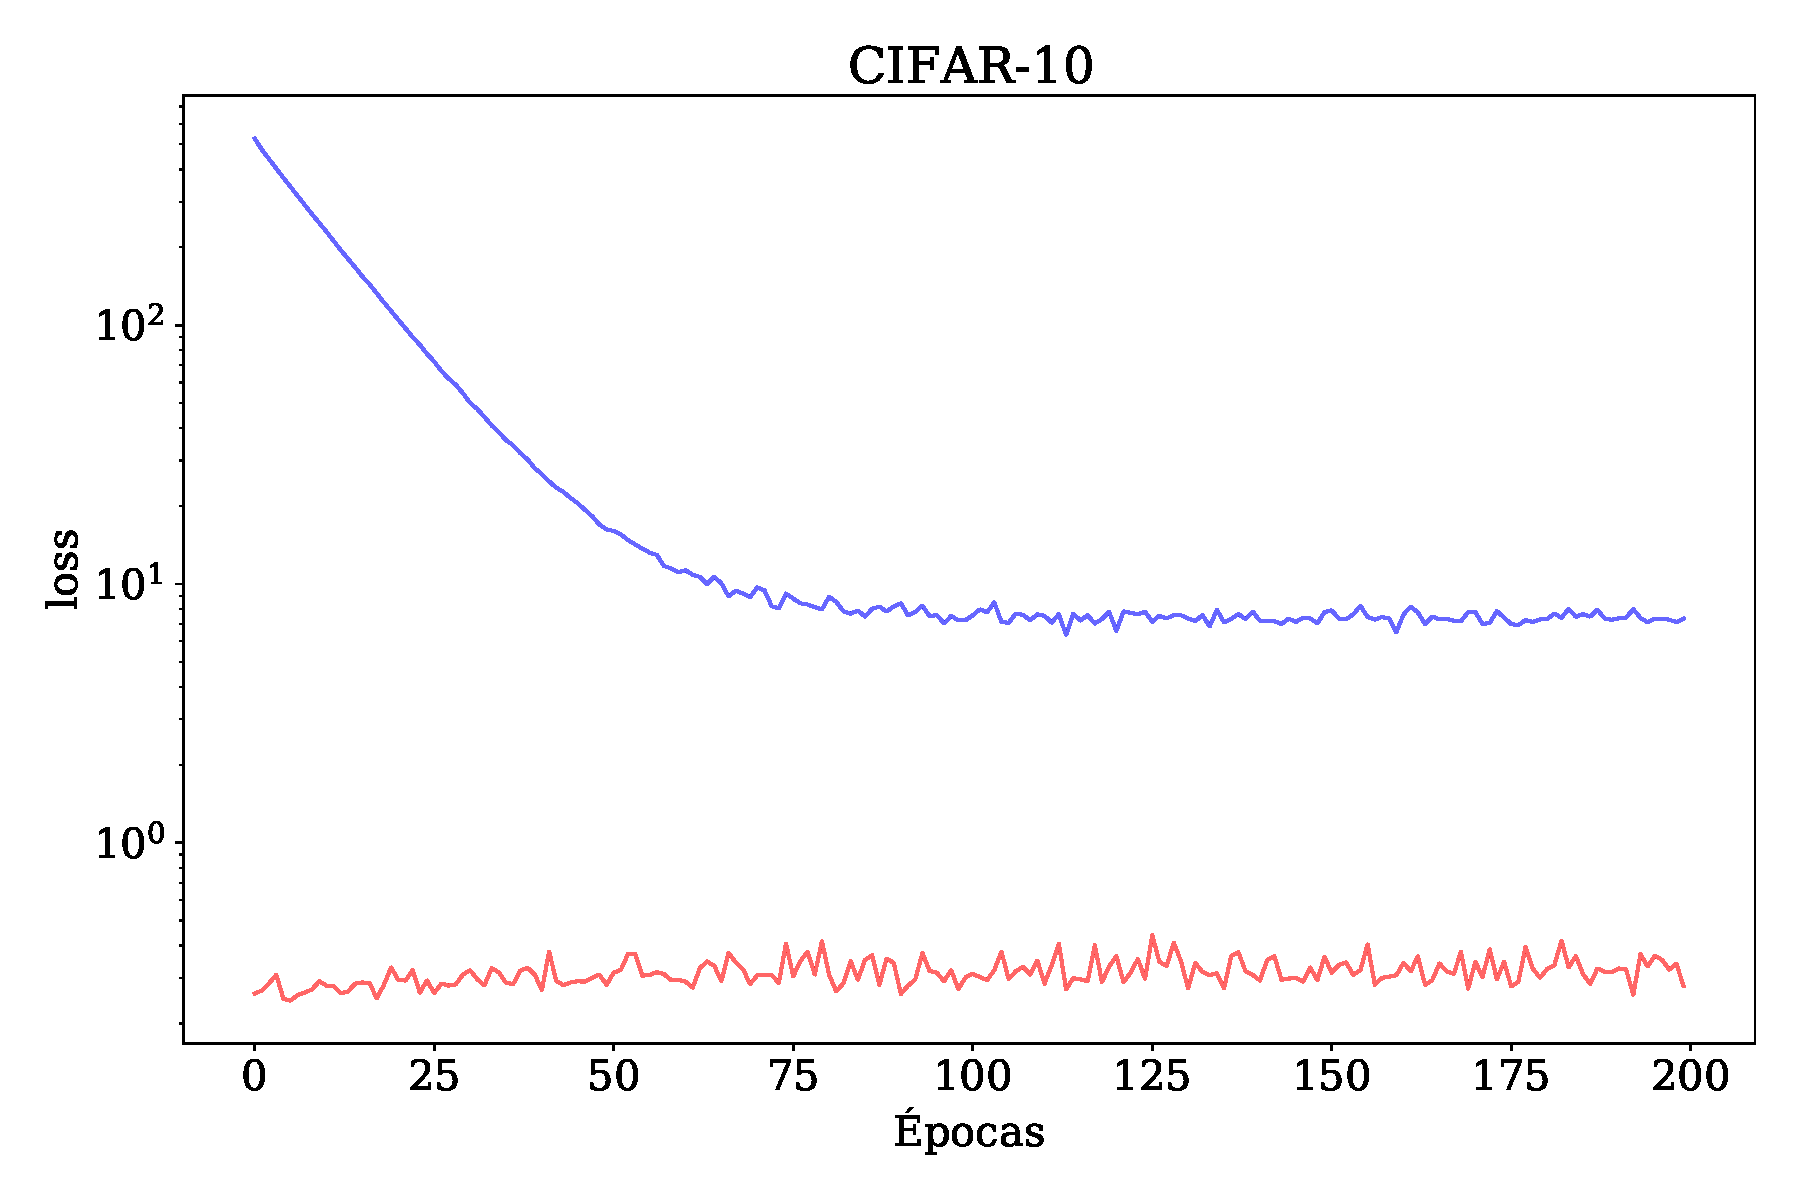
\includegraphics[width=0.5\textwidth]{../../ejer_5_CIFAR-10_los.pdf}
    \caption{Pérdida en función de las épocas de los algoritmos sobre el CIFAR-10}
    \label{fig:ejer5_cifar10_loss}
\end{figure} 


\end{document}